\chapter{SAF microarchitecture taxonomy}

In this work, SAF microarchitecture categorization is intended to facilitate communication of general design principles, very early planning discussions among designers, and design-space exploration of possible SAF microarchitectures. \todo{It is important to set up a systematic way of describing components and how they connect to each other. Later, we use this taxonomy as the basis of a set of tools for inferring the SAF microarchitecture design and modeling its energy, area and latency.} \\
%
A sufficiently expressive taxonomic framework encompasses SAF microarchitecture designs seen in the literature and may also express design not yet developed, enabling improvements on existing work. However a highly detailed and expressive representation of microarchitecture as, i.e., RTL, is not ideal because the design-space is huge and difficult to describe or constrain, or even to extract general design principles from. Existing architectural modeling tools face similar problems with exponential growth in the space of possible designs as the language for describing designs becomes more expressive, which they address by (1) limiting to a finite set of architectural primitives (i.e. SRAM, MAC, etc.)\cite{timeloop}, (2) supporting hierarchical component representations built out of primitives \cite{accelergy} such that a small primitive library enables a large space of designs, (3) parameterizing component categories with a concise set of attributes that are sufficient to narrow down an implementation \cite{accelergy}, (4) describing optimizations (i.e. SAFs as described in \cite{sparseloop}) as annotations on architectural components which themselves have attributes sufficient to describe the optimization strategy, and (5) producing frameworks which are extensible to help designers to concisely express key design-specific components. \todo{Antipattern - paper on specific microarchitectures only.} \\
%
This work addresses the challenge of describing SAF microarchitectures in an expressive but concise way, which is easily extensible by users. Ideally a designer could express many useful SAF microarchitectures as a netlist or schematic, not of logic gates, but of connections between higher-level ``SAF primitive components'' which recur frequently across published SAF microarchitecture designs. Components are further parameterized with attributes sufficient to narrow down the general energy, area and latency scaling behavior of the underlying implementation. To that end, the conceptual framework developed in this work consists of
%
\begin{itemize}
    \item A taxonomic categorization of SAF primitives
    \item For each taxonomic primitive, a set of attributes sufficient to narrow down the general type of microarchitecture implementation as well as the scaling behavior of energy, area and latency
    \item For each SAF described in \cite{sparseloop} (format, gating, skipping), a feasible set possible topologies for building the SAF microarchitecture out of SAF primitives
    \item For each SAF, a set of attributes which are sufficient to narrow down the appropriate SAF microarchitecture out of the feasible set. This set includes at least the attributes of the SAF itself (i.e. type of action optimization, or choice of representation format), as well as other attributes specific to the SAF microarchitecture.
\end{itemize}

\section{Primitive components}

This section will overview the taxonomy of microarchitectural primitive components considered in this work.

\subsection{Metadata parsers}

\begin{figure}[H]
    \centering
    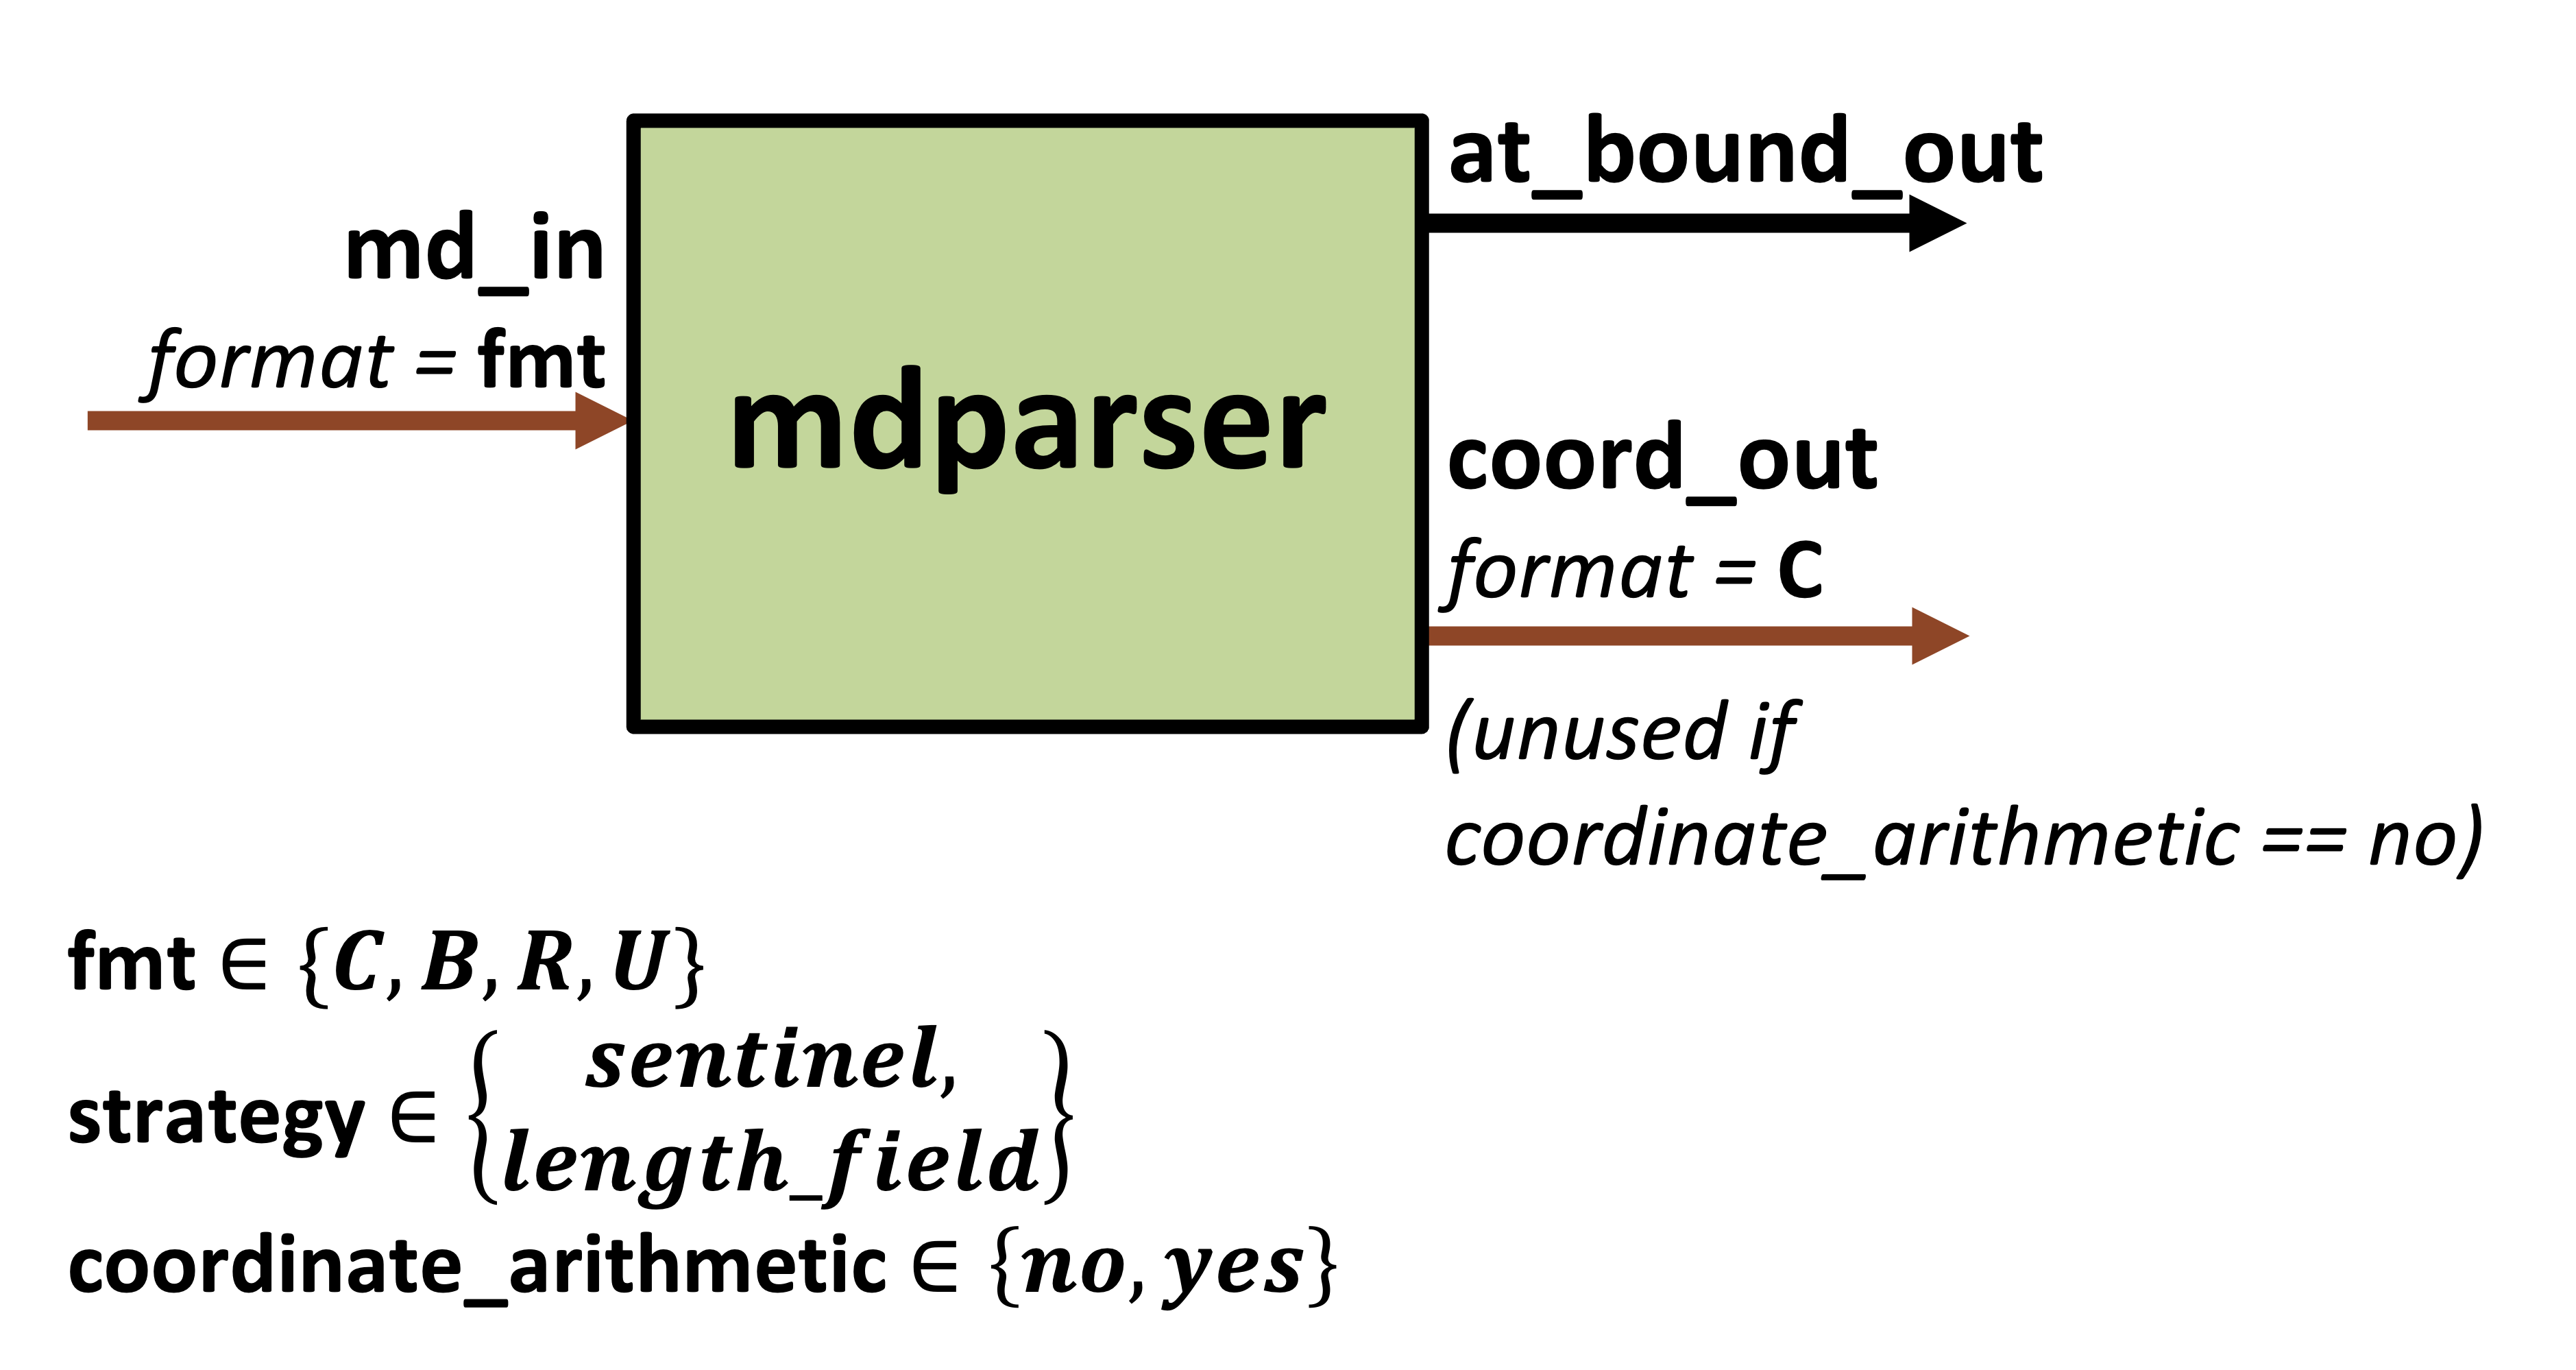
\includegraphics[width=0.95\textwidth]{figures/mdparser.png}
    \caption{Metadata parser primitive component template.}
    \label{fig:mdparser}
\end{figure}

\begin{table}[H]
\centering
\begin{tabular}{lll}
\toprule
 format   & strategy       & coordinate\_arithmetic   \\
\midrule
 U        & sentinel & no\_arithmetic                \\
 U        & sentinel & yes\_arithmetic                 \\
 U        & length\_field & no\_arithmetic              \\
 U        & length\_field & yes\_arithmetic             \\
 C        & sentinel & no\_arithmetic                \\
 C        & sentinel & yes\_arithmetic                 \\
 C        & length\_field & no\_arithmetic              \\
 C        & length\_field & yes\_arithmetic             \\
 B        & sentinel & no\_arithmetic                  \\
 B        & sentinel & yes\_arithmetic                 \\
 B        & length\_field & no\_arithmetic              \\
 B        & length\_field & yes\_arithmetic             \\
\bottomrule
\end{tabular}
\caption{Specializations of metadata parsers.}
\label{tab:MetadataParser_specializations}
\end{table}

\subsection{Position generators}

\subsubsection{Single position generators}

\begin{figure}[H]
    \centering
    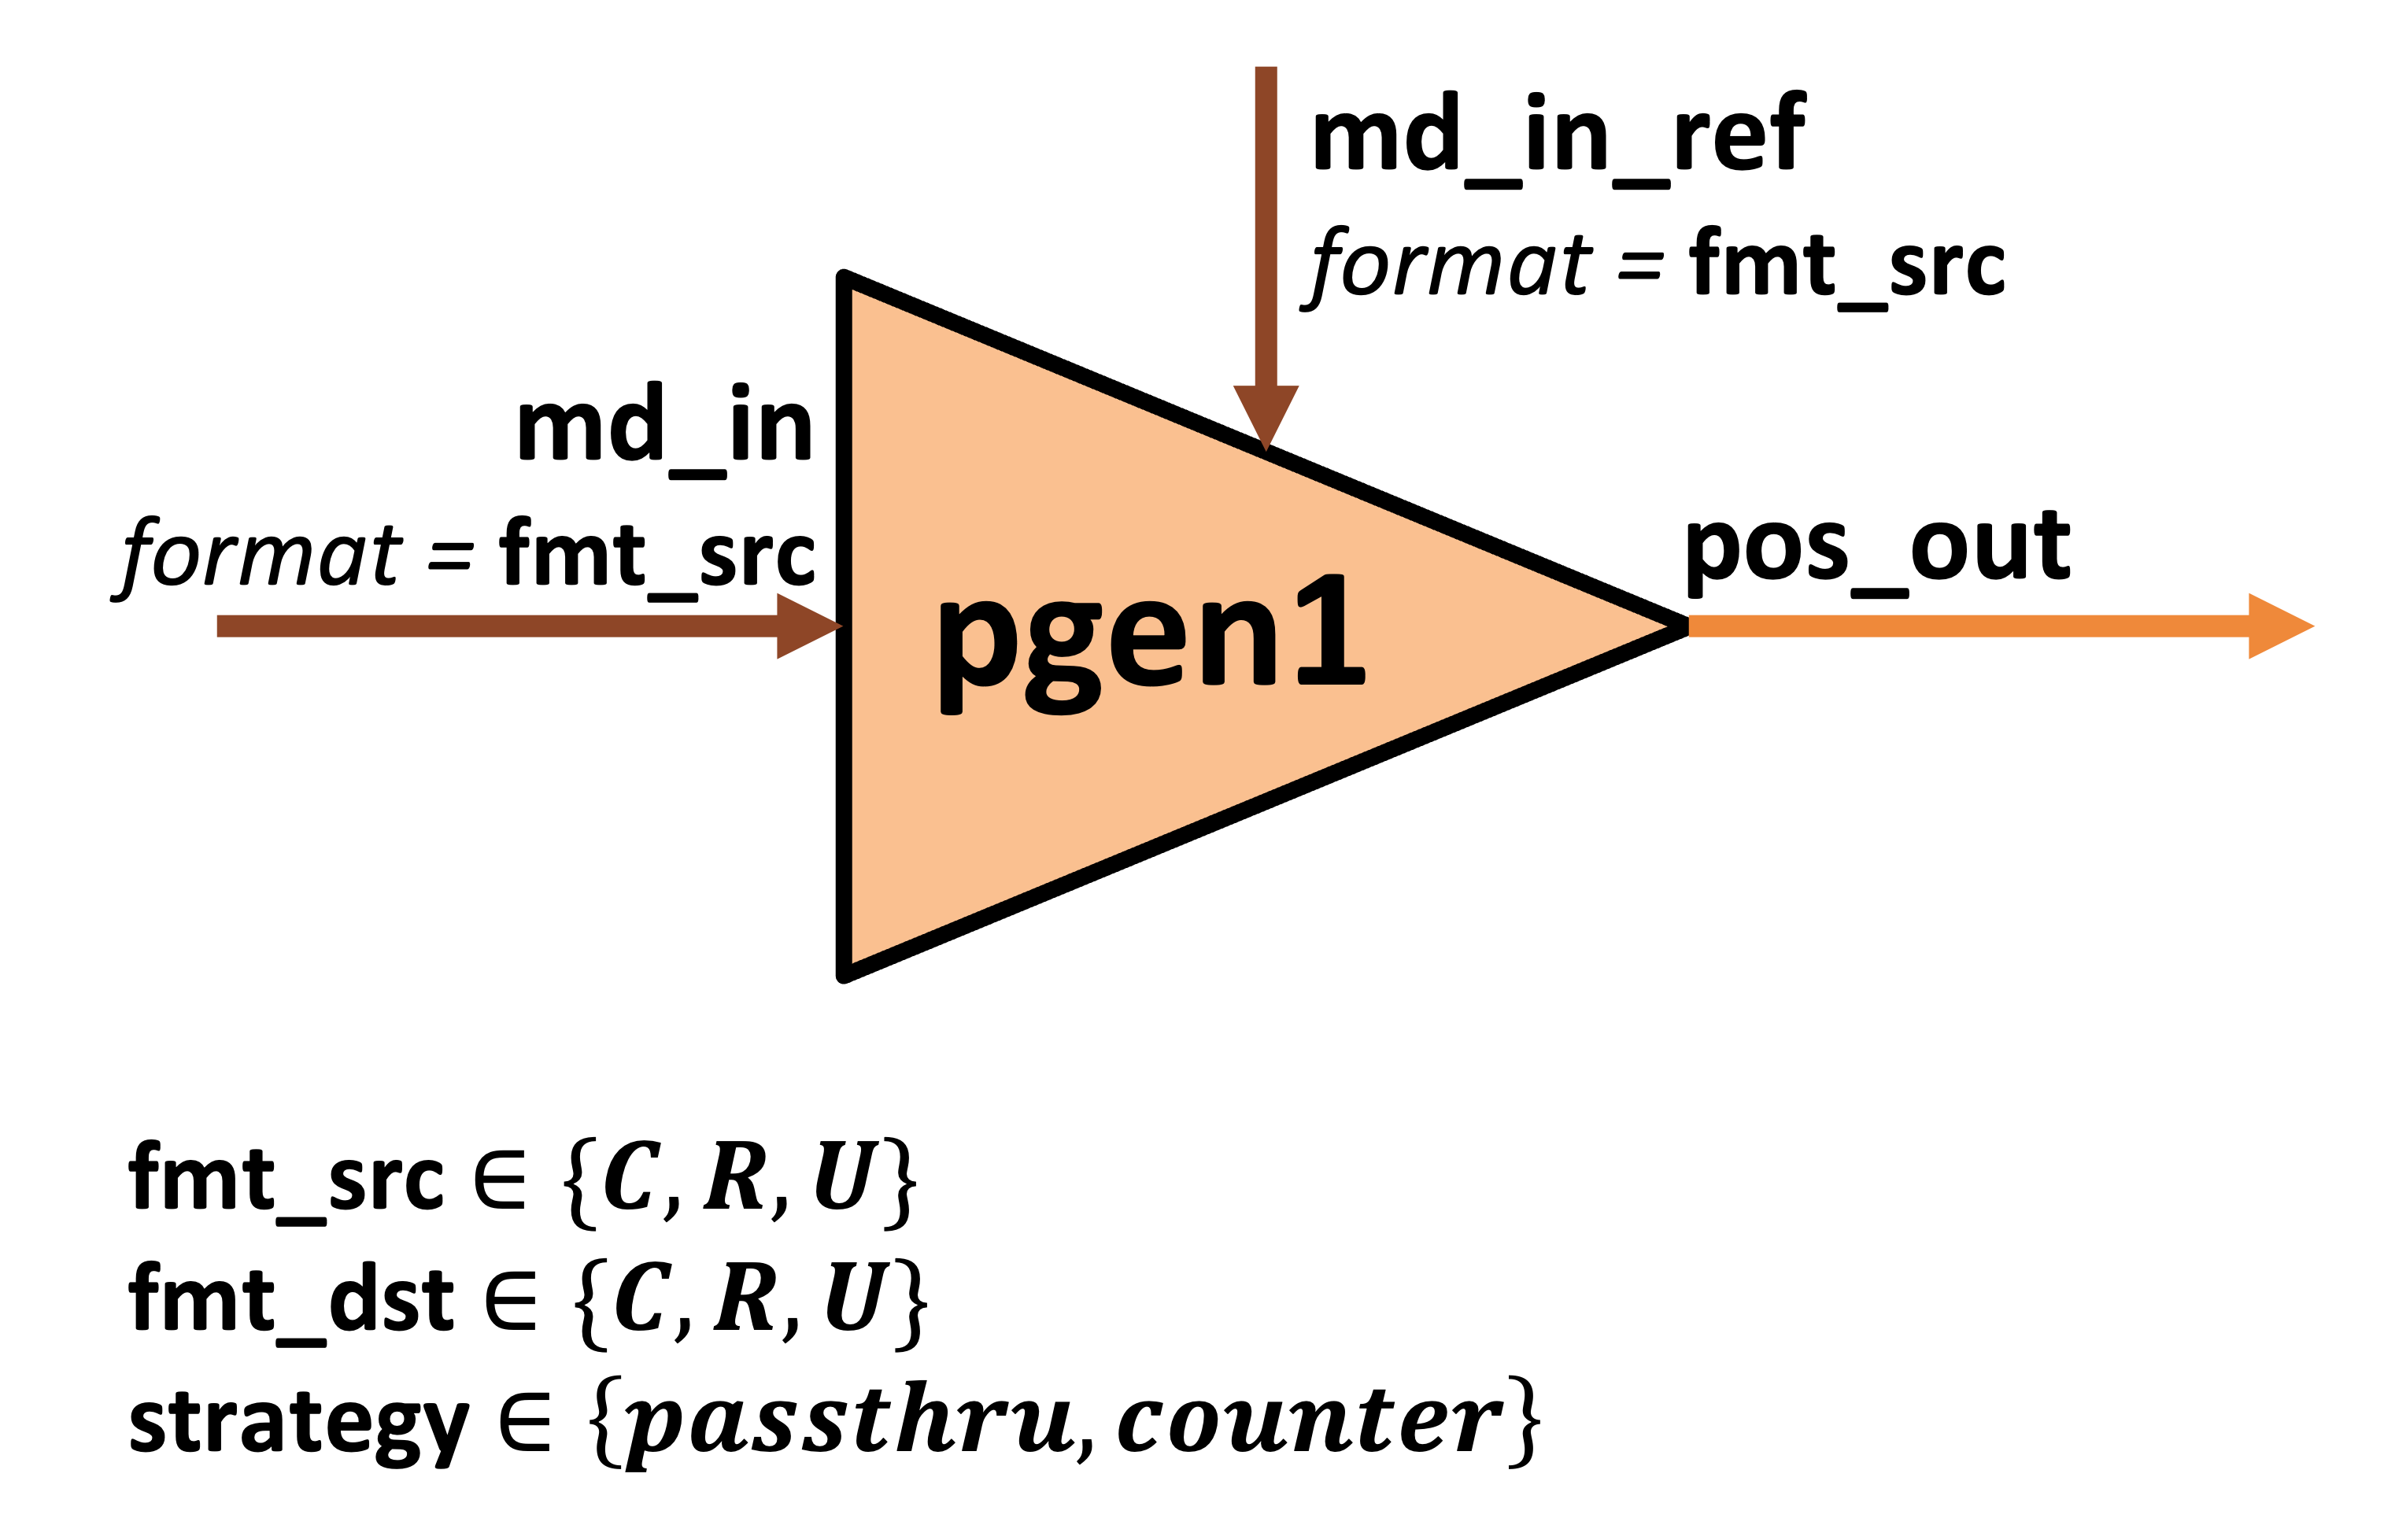
\includegraphics[width=0.95\textwidth]{figures/pgen1.png}
    \caption{Single position generator primitive component template.}
    \label{fig:pgen1}
\end{figure}

\begin{table}[H]
\centering
\begin{tabular}{lll}
\toprule
 format\_src   & format\_dst   & strategy    \\
\midrule
 C            & U            & passthrough \\
 C            & C            & counter     \\
\bottomrule
\end{tabular}
\caption{Specializations of single position-generator}
\label{tab:SinglePositionGenerator_specializations}
\end{table}

\subsubsection{Dual position generators}

\begin{figure}[H]
    \centering
    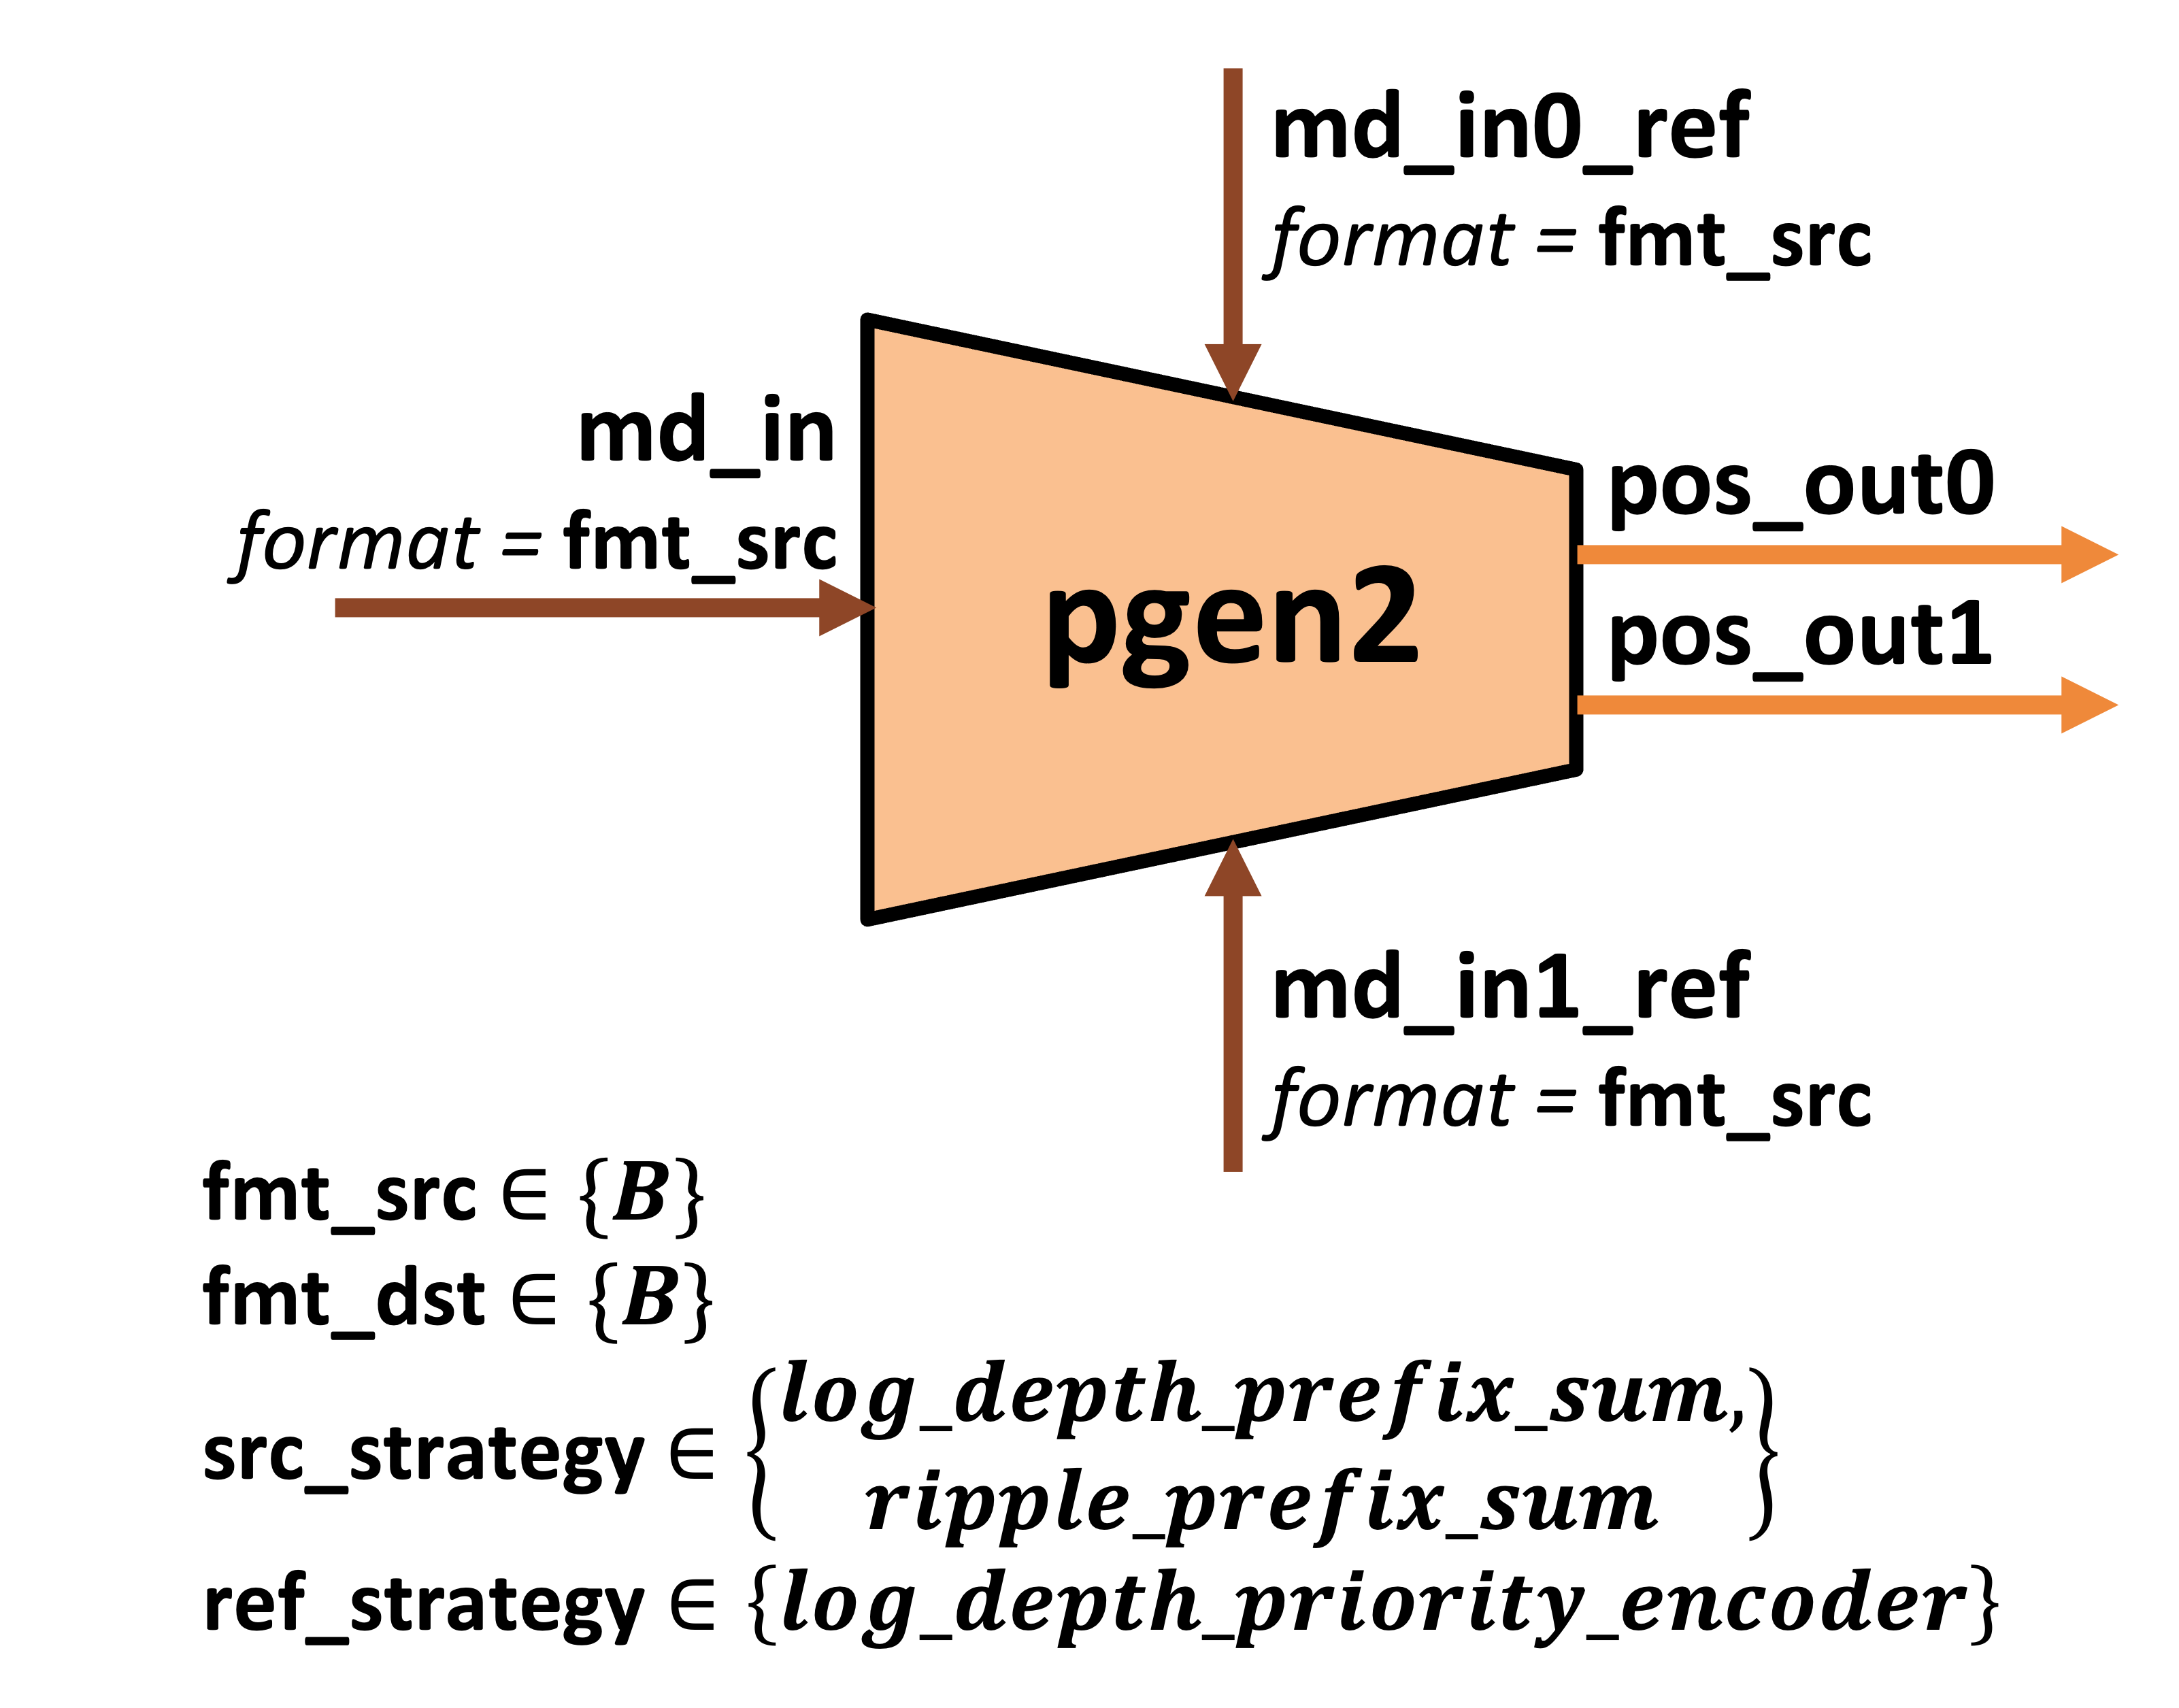
\includegraphics[width=0.95\textwidth]{figures/pgen2.png}
    \caption{Dual position generator primitive component template.}
    \label{fig:pgen2}
\end{figure}

\begin{table}[H]
\centering
\begin{tabular}{llll}
\toprule
 format\_src   & format\_dst   & source\_strategy        & reference\_strategy             \\
\midrule
 B            & B            & ripple\_prefix\_sum      & parallel\_dec2\_priority\_encoder \\
 B            & B            & kogge\_stone\_prefix\_sum & parallel\_dec2\_priority\_encoder \\
\bottomrule
\end{tabular}
\caption{Specializations of dual position generator}
\label{tab:DualPositionGenerator_specializations}
\end{table}

\subsection{Intersection units}

\subsubsection{Leader-follower intersection units}

\begin{figure}[H]
    \centering
    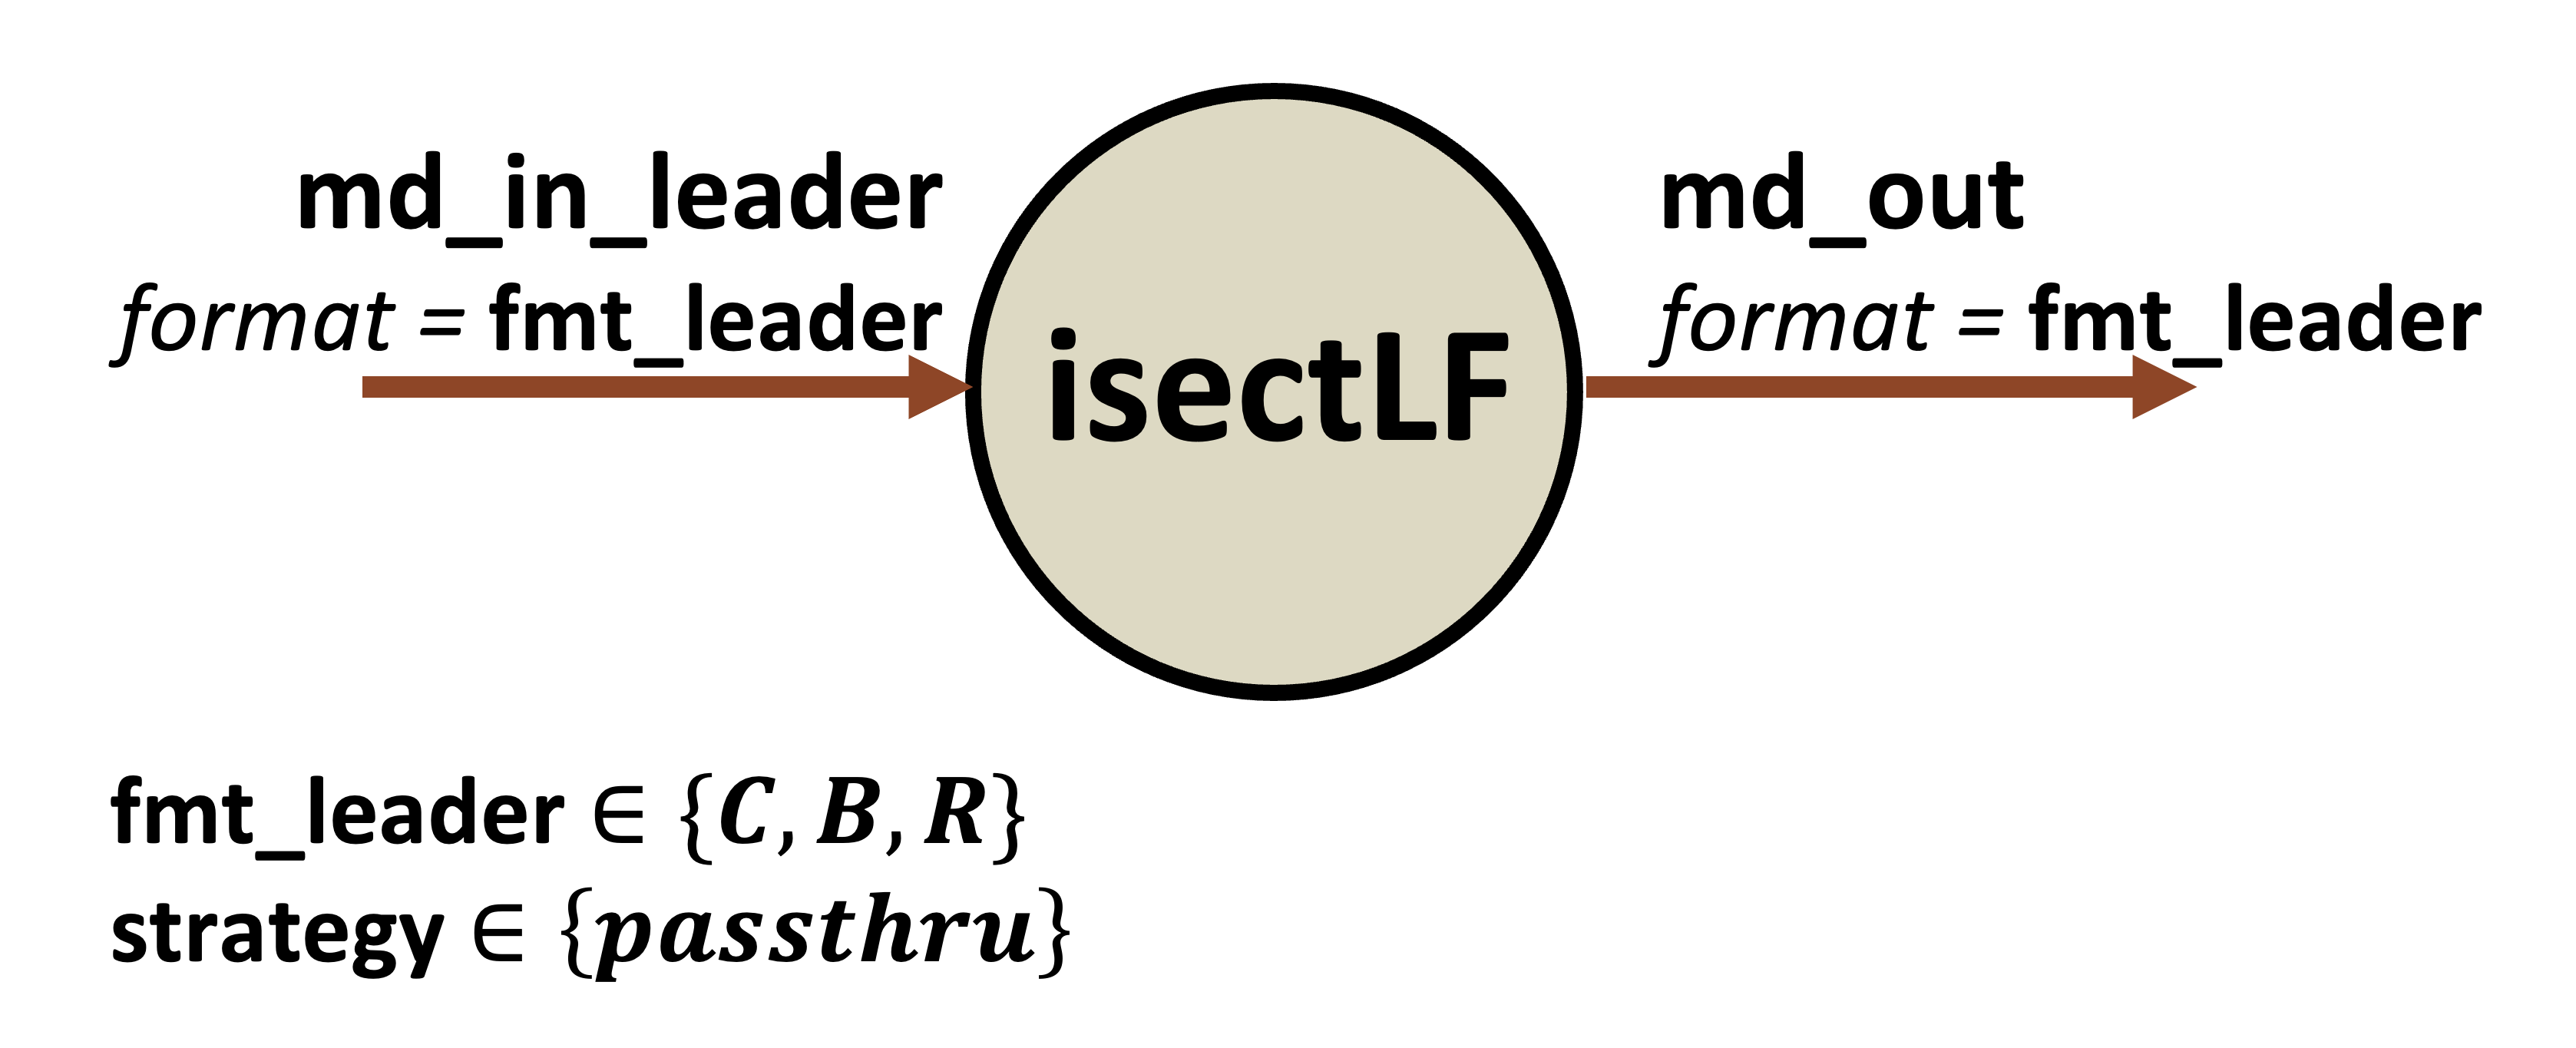
\includegraphics[width=0.95\textwidth]{figures/isectlf.png}
    \caption{Leader-follower intersection primitive component template.}
    \label{fig:isectlf}
\end{figure}

\begin{table}[H]
\centering
\begin{tabular}{ll}
\toprule
 format\_leader   & strategy    \\
\midrule
 C               & passthrough \\
 B               & passthrough \\
 R               & passthrough \\
\bottomrule
\end{tabular}
\caption{Specializations of leader-follower intersection.}
\label{tab:IntersectionLeaderFollower_specializations}
\end{table}

\subsubsection{Bidirectional intersection units}

\begin{figure}[H]
    \centering
    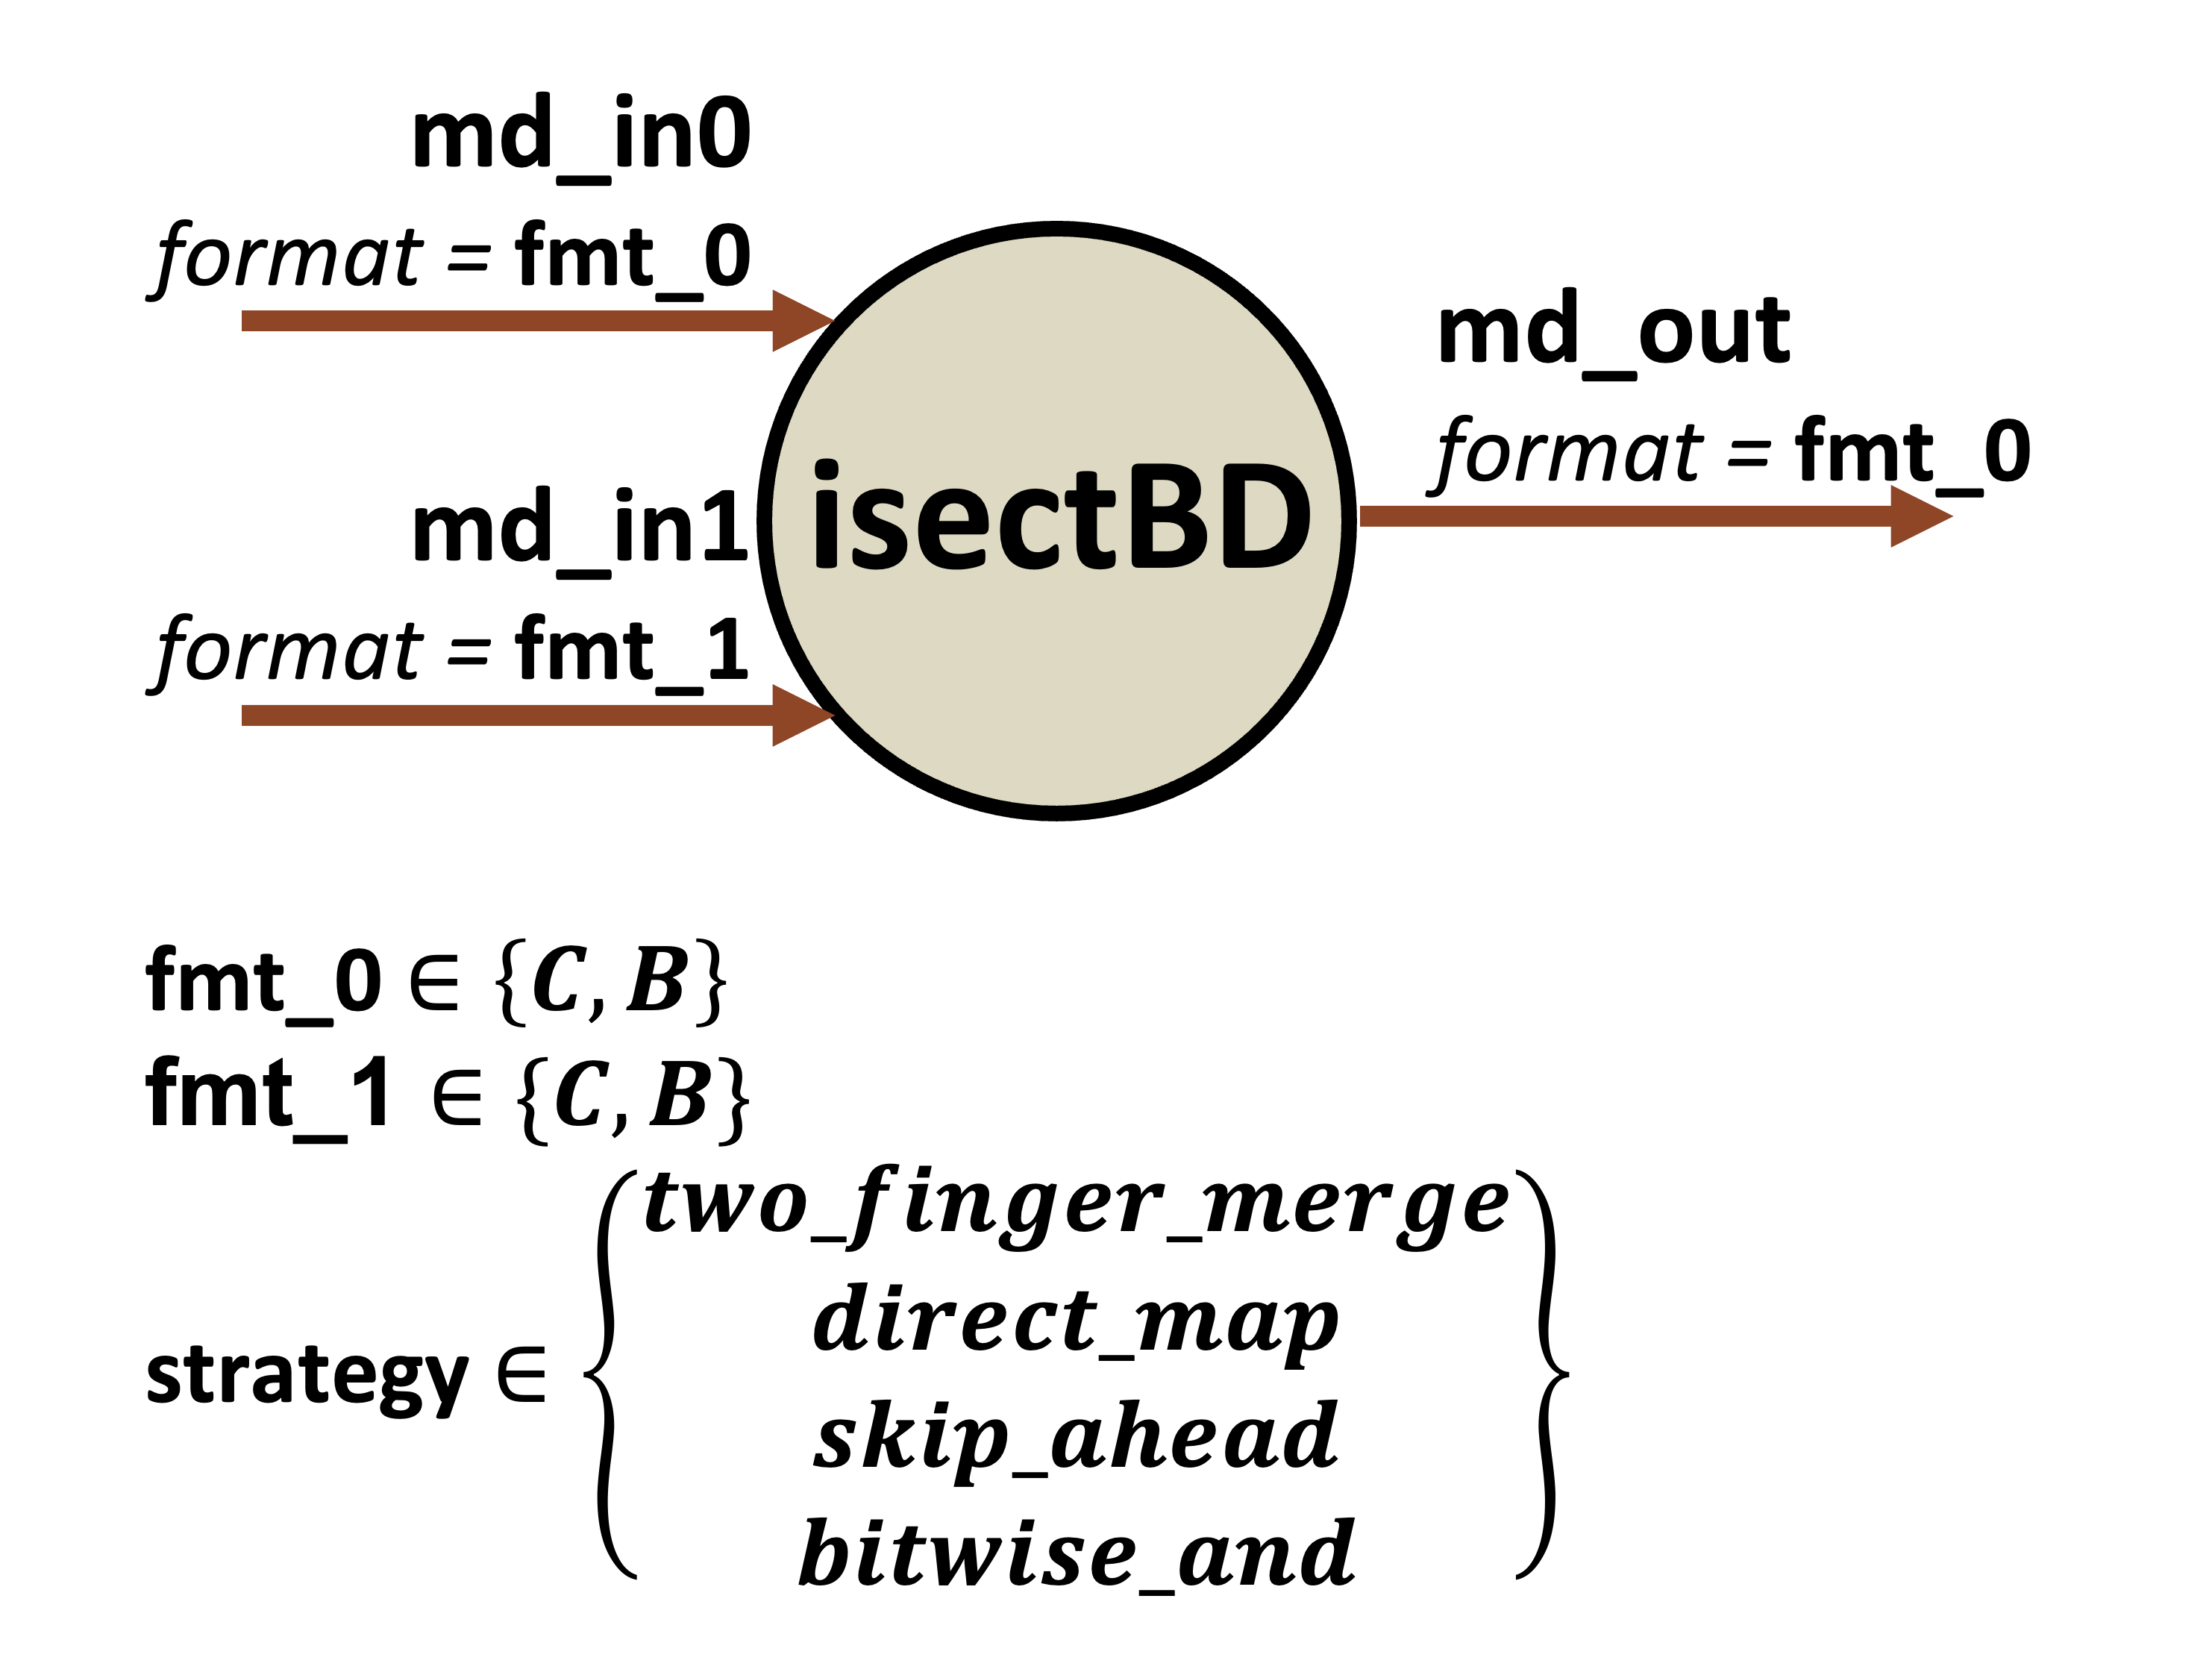
\includegraphics[width=0.95\textwidth]{figures/isectbd.png}
    \caption{Bidirectional intersection primitive component template.}
    \label{fig:isectbd}
\end{figure}

\begin{table}[H]
\centering
\begin{tabular}{lll}
\toprule
 format\_0   & format\_1   & strategy         \\
\midrule
 C          & C          & two\_finger\_merge \\
 C          & C          & skip\_ahead       \\
 C          & C          & direct\_map       \\
 B          & B          & bitwise\_and      \\
\bottomrule
\end{tabular}
\caption{Specializations of bidirectional intersection.}
\label{tab:IntersectionBidirectional_specializations}
\end{table}

\subsection{Fill optimizers}

\begin{figure}[H]
    \centering
    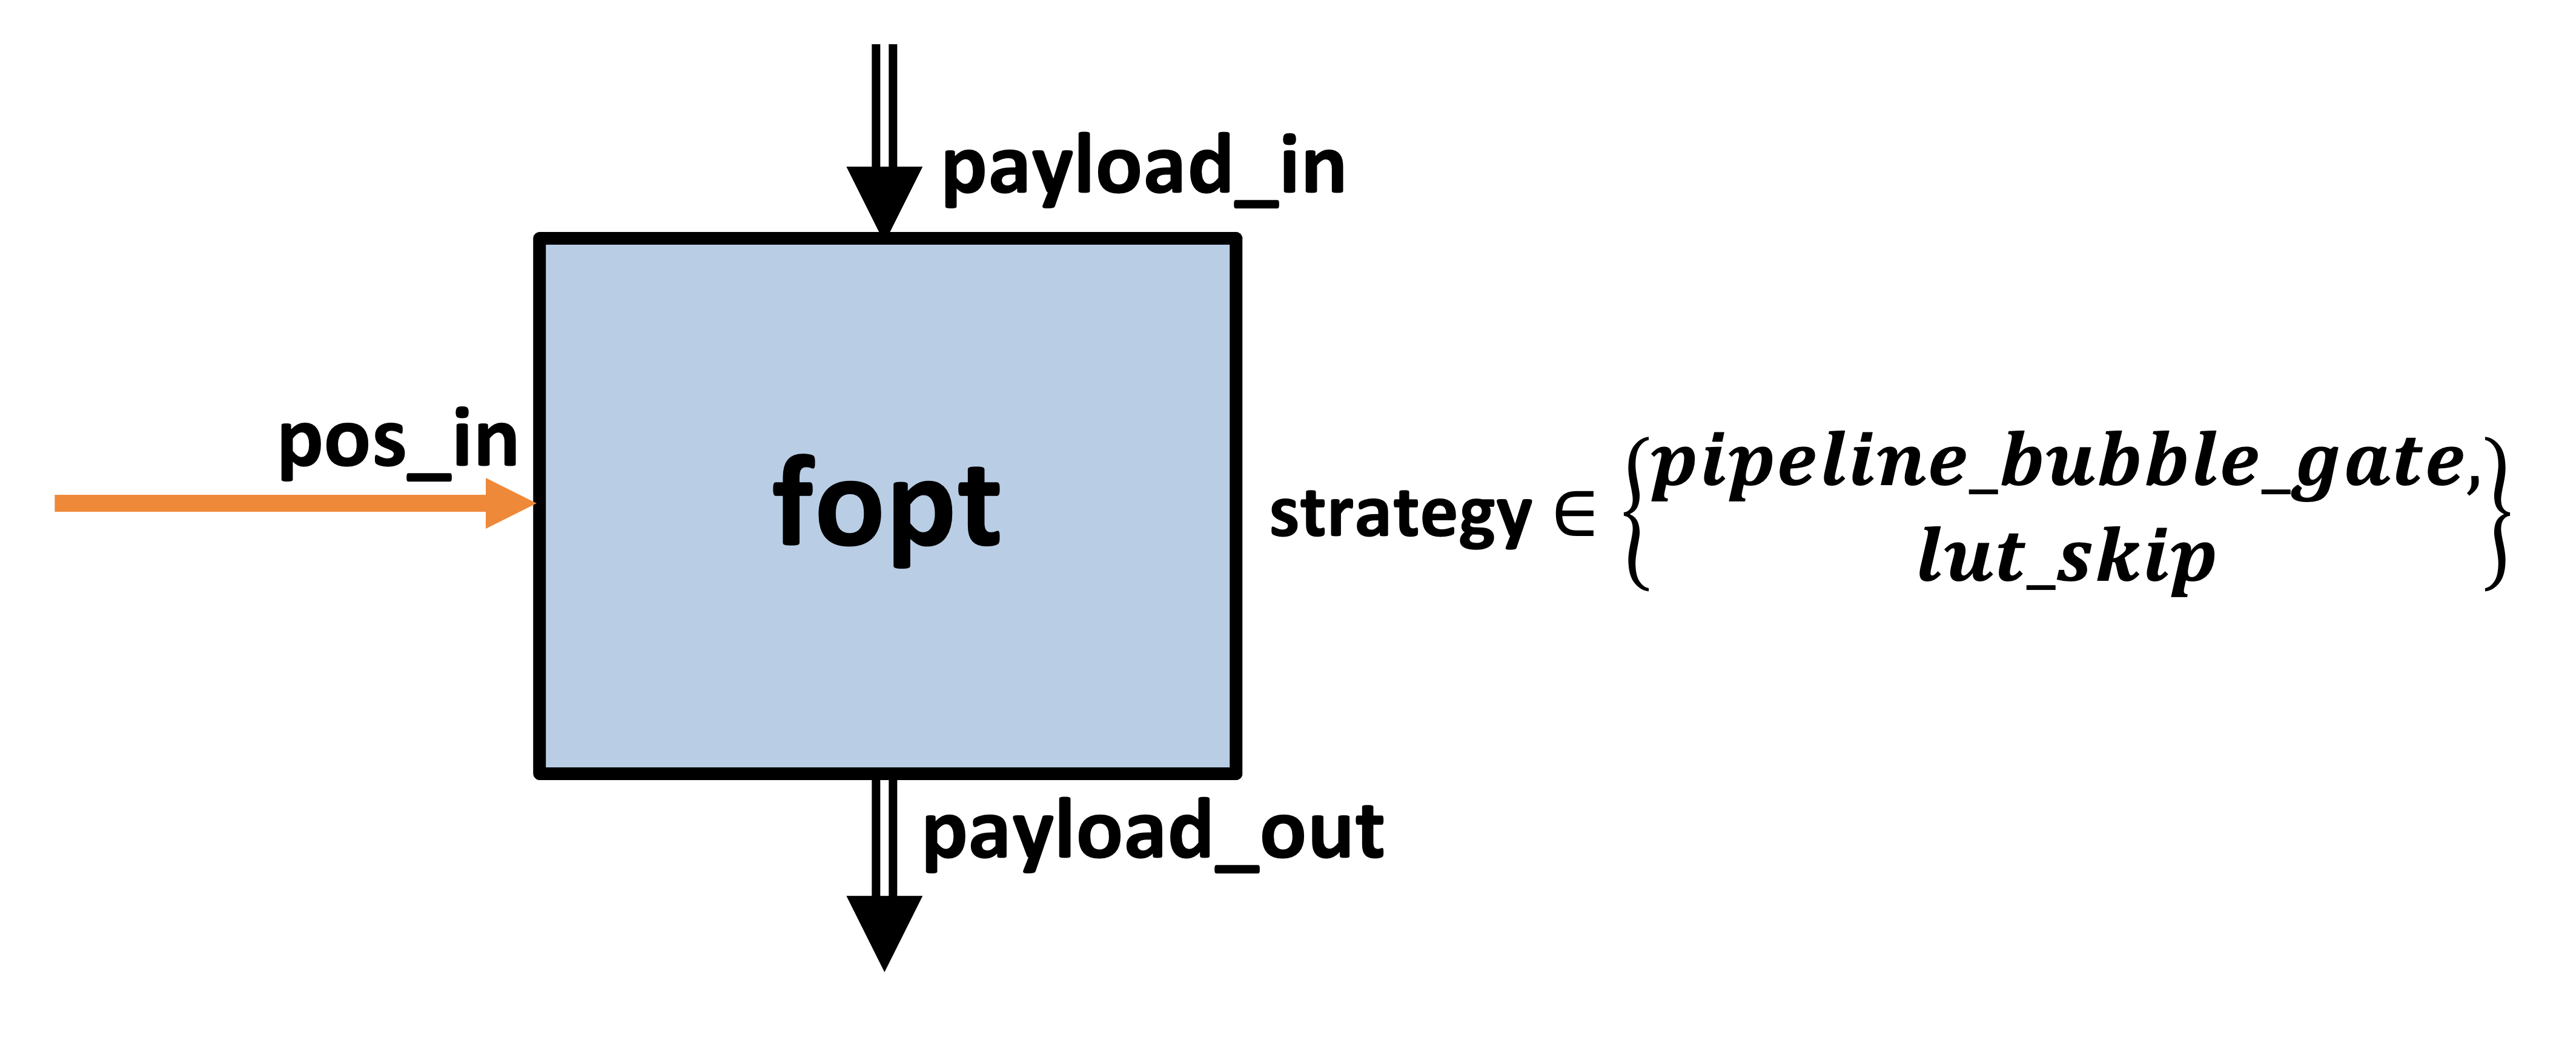
\includegraphics[width=0.95\textwidth]{figures/fopt.png}
    \caption{Fill optimizer primitive component template. The fill optimizer's (fopt's) method for discarding payload fills - as well as the interface between the fopt and the payload stream - is highly implementation-dependent, thus the fopt template does not have a ``payload'' interface. The red dotted line from fopt to payload stream is a visual cue for which payload stream is being optimized, but in actuality \textit{pos\_in} is the only interface port defined for this primitive component template.}
    \label{fig:fopt}
\end{figure}

\begin{table}[H]
\centering
\begin{tabular}{l}
\toprule
 strategy             \\
\midrule
 pipeline\_bubble\_gate \\
 lut\_skip             \\
\bottomrule
\end{tabular}
\caption{Specializations of fill optimizer}
\label{tab:FillOptimizer_specializations}
\end{table}

\section{SAF microarchitectures}

This section will overview the taxonomy of SAF microarchitectures considered in this work. SAF microarchitectures implement SAFs. Though not a requirement, in practice all SAF microarchitectures considered in this work were well-described as compound components, and conversely the only compound components modeled in this work happen to be SAF microarchitectures.

\subsection{Format microarchitectures}

\begin{figure}[H]
    \centering
    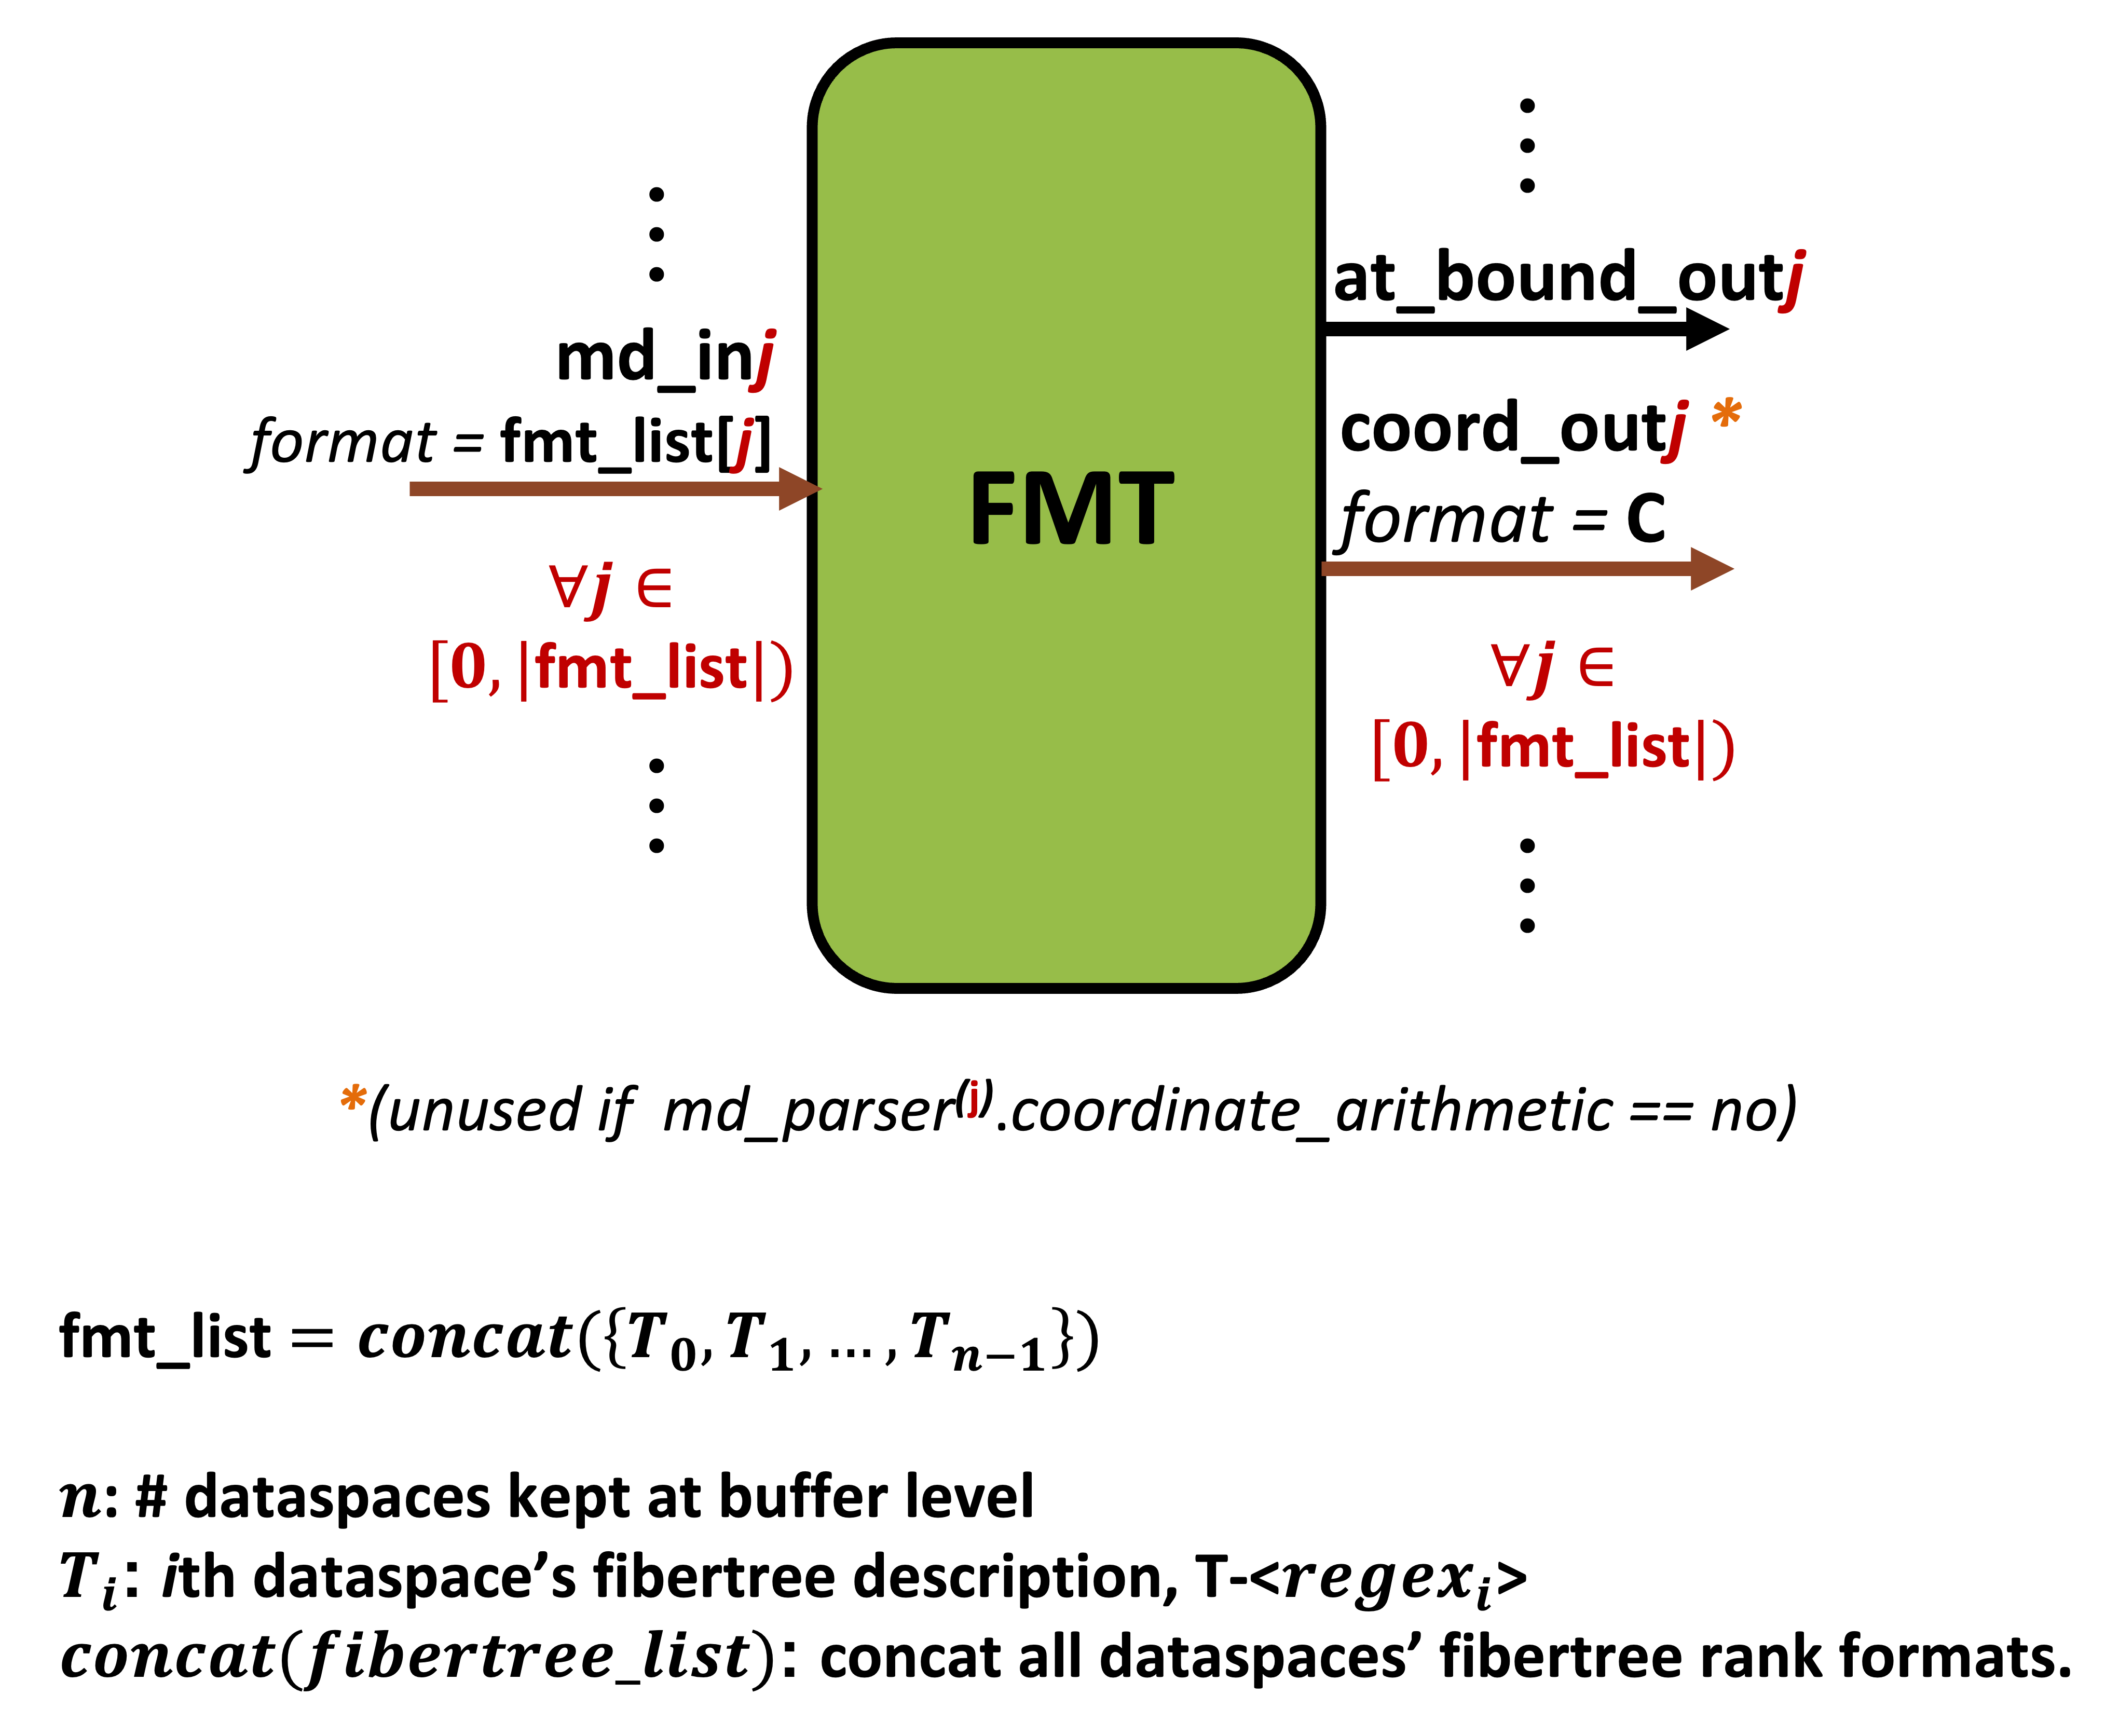
\includegraphics[width=0.95\textwidth]{figures/FMT.png}
    \caption{Format microarchitecture compound component template. If an architectural buffer has a format SAF, a format microarchitecture must be bound to it. The fmt\_list parameter expects a list of rank formats. The architectural buffer keeps\cite{timeloop} one or more dataspaces\cite{timeloop}, at least one of which exploits a format SAF. fmt\_list is assumed to have been derived from concatenating the fiber representation regexes\cite{szebook} for all kept dataspaces' fibertrees, excluding dataspaces which do not exploit a format SAF.}
    \label{fig:FMT}
\end{figure}

%\begin{table}[H]
%\centering
%\begin{tabular}{l}
%\toprule
% fibertree   \\
%\midrule
% *           \\
%\bottomrule
%\end{tabular}
%\caption{Specializations of format microarchitecture}
%\label{tab:format_microarchitecture_specializations}
%\end{table}

\begin{figure}[H]
    \centering
    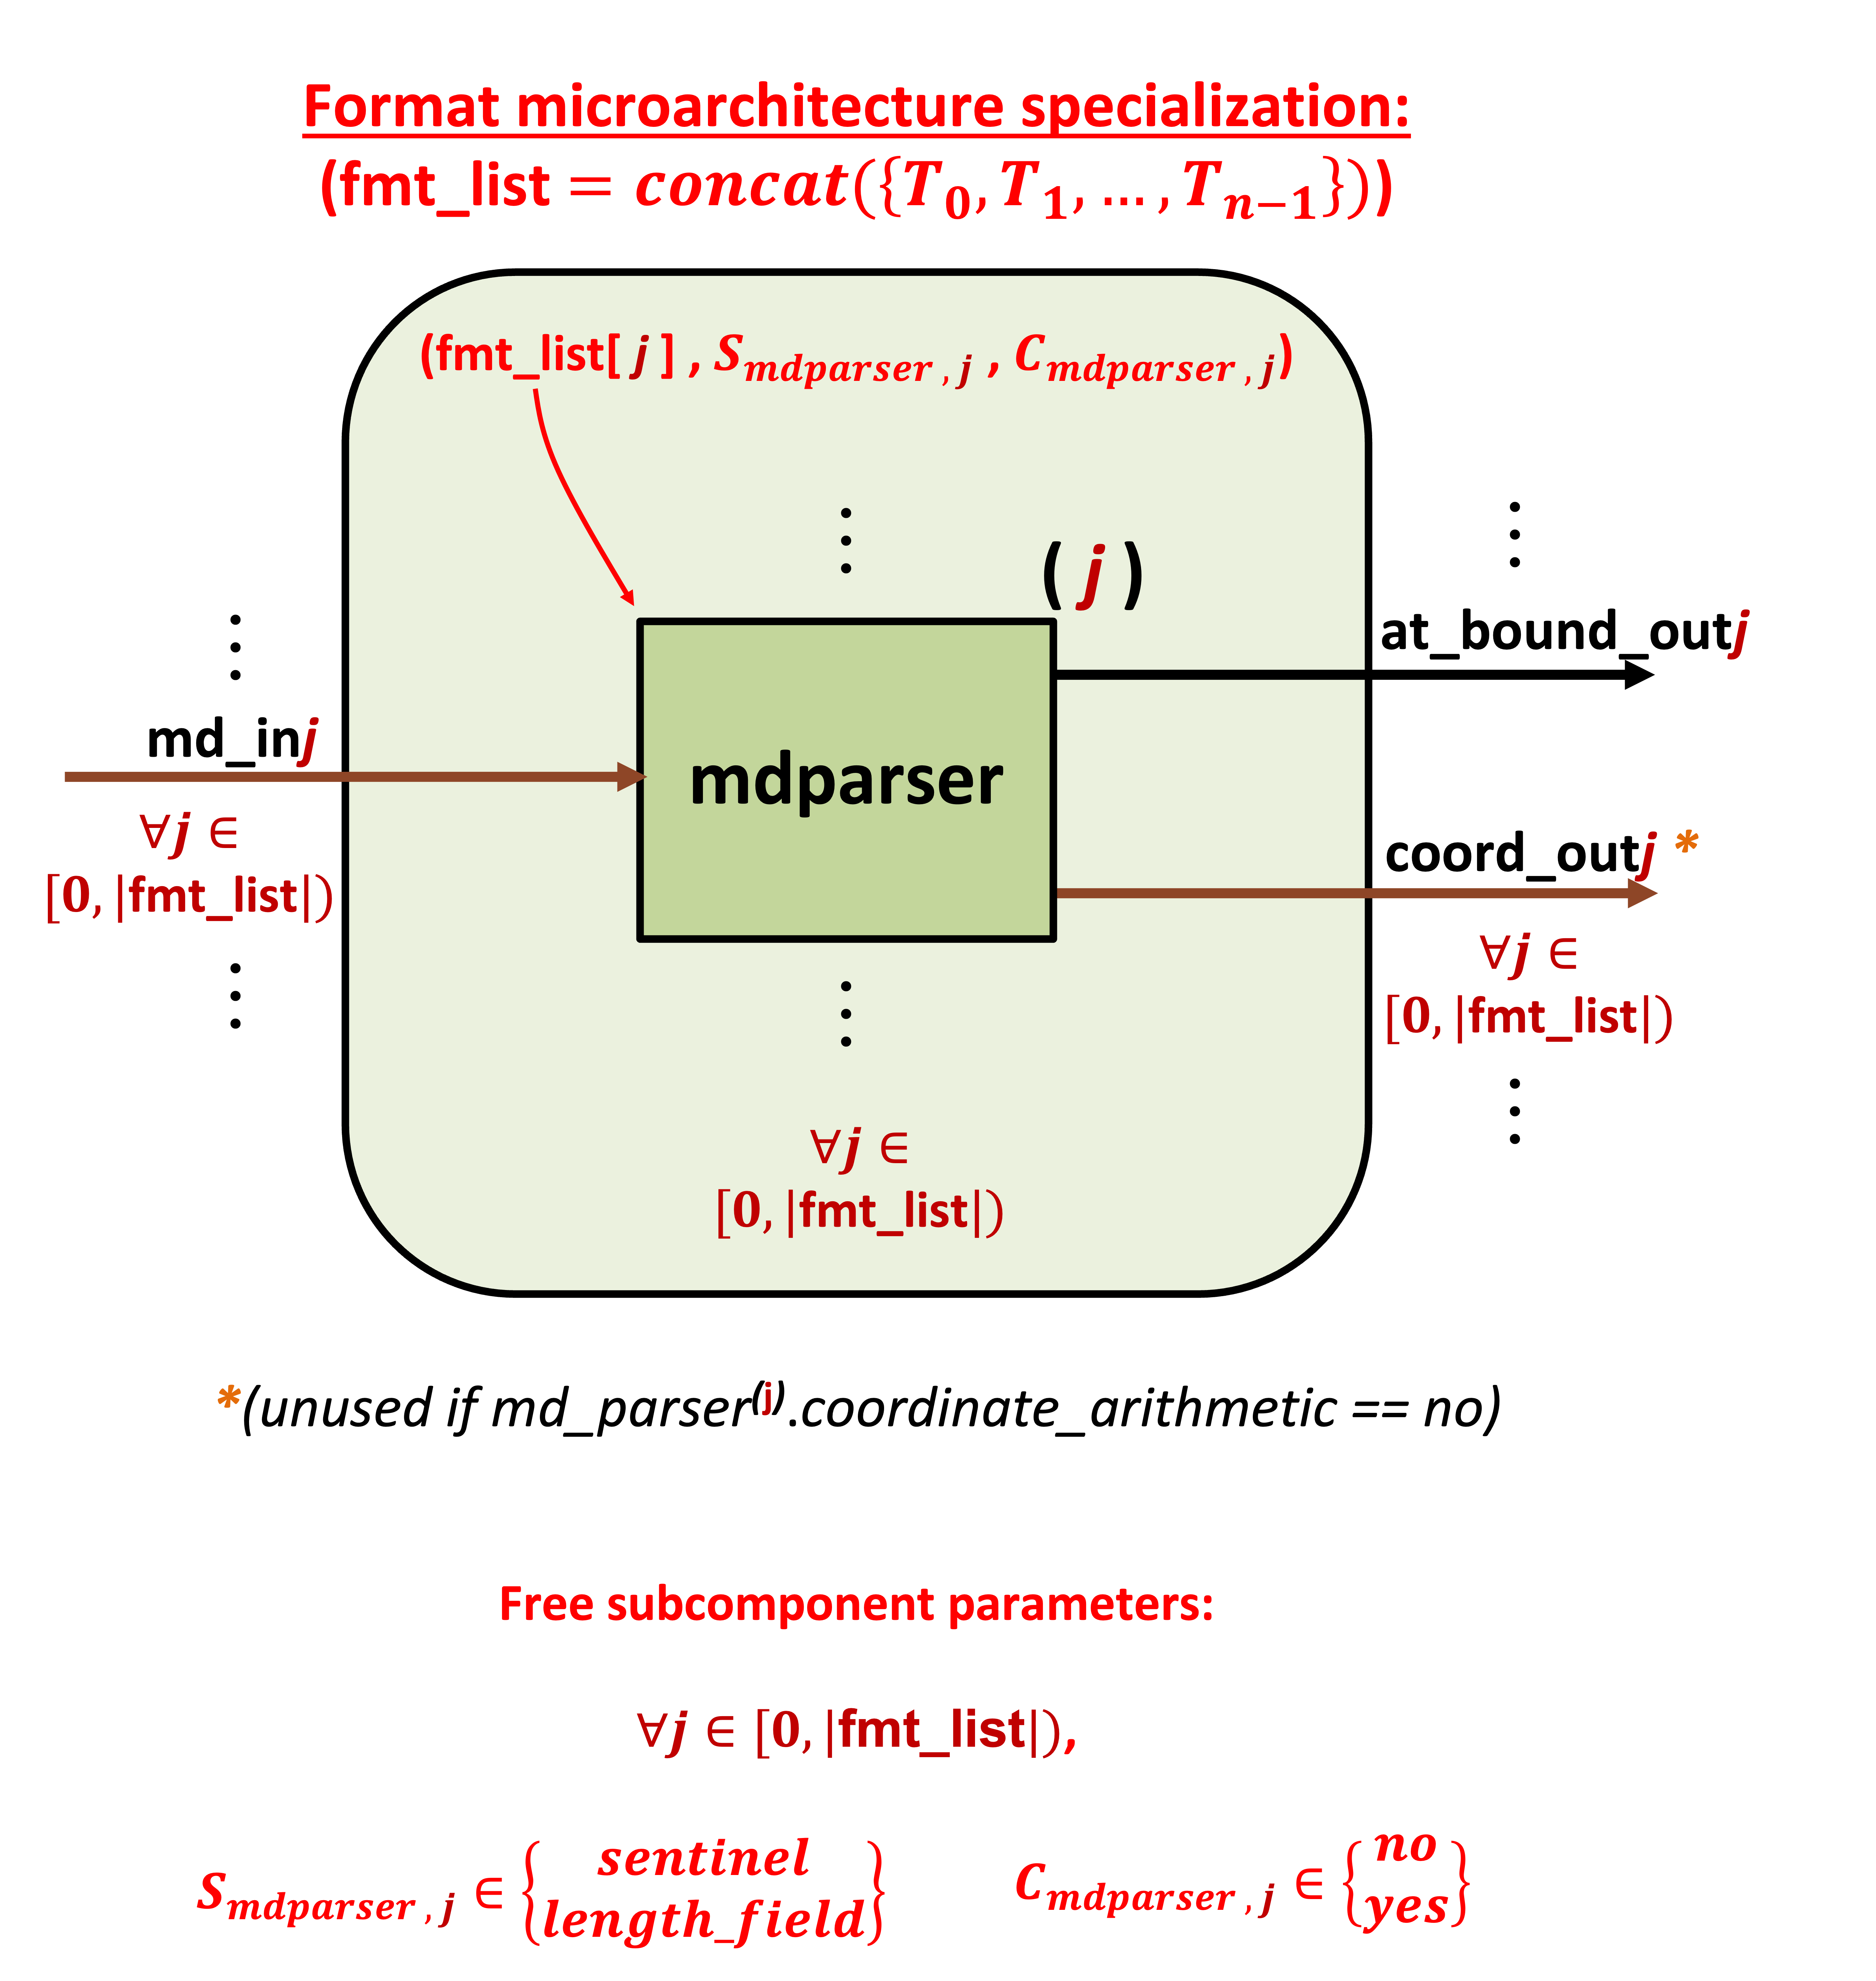
\includegraphics[width=0.95\textwidth]{figures/FMT_all.png}
    \caption{Format microarchitecture implementation topology. Every rank, in every fibertree, in every kept dataspace which is subject to a format SAF for a given buffer, has a corresponding metadata parser in the format microarchitecture topology. This implementation topology is universal for format microarchitectures regardless of the specific \textit{fmt\_list} parameter value. Each metadata parser subcomponent, however, has two free parameters. Setting \textit{coordinate\_arithmetic = no} for the $j$th metadata parser, means that that format microarchitecture will not support coordinate arithmetic for the corresponding fibertree rank. This can conserve resources i.e. if the rank is being contracted anyway.}
    \label{fig:FMT_all}
\end{figure}

\subsection{Skipping microarchitectures}

\begin{figure}[H]
    \centering
    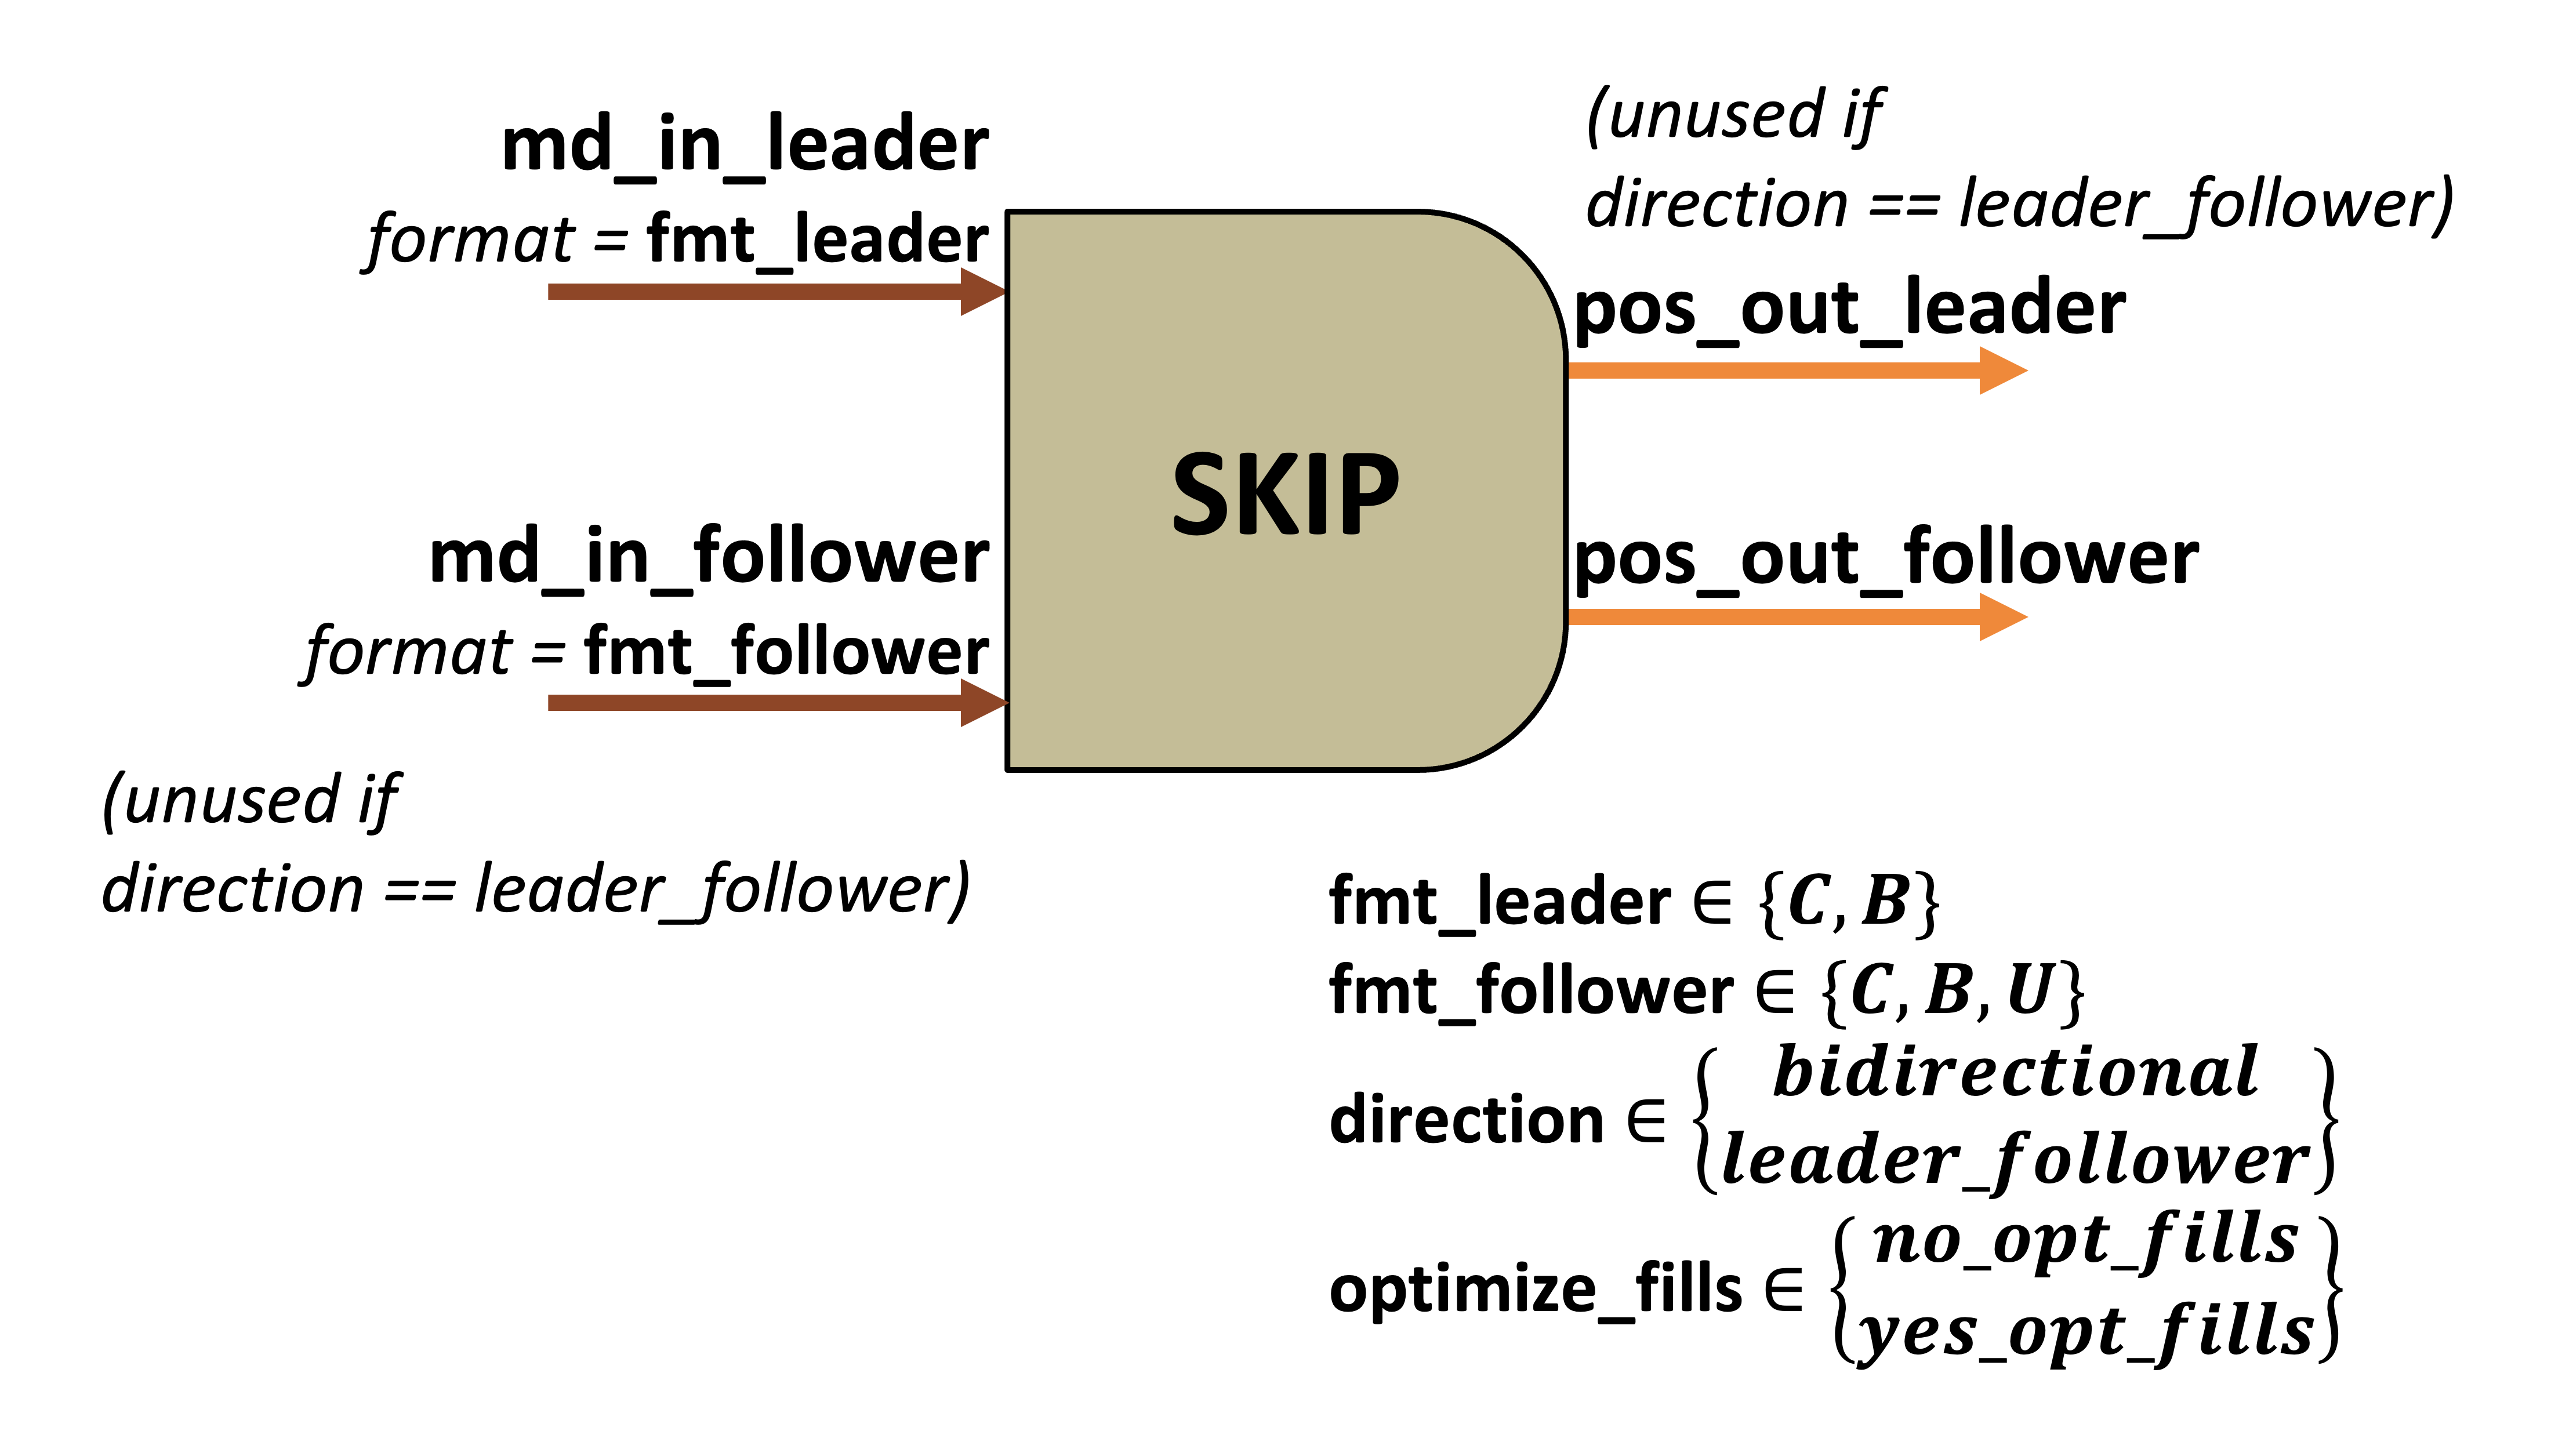
\includegraphics[width=0.95\textwidth]{figures/SKIP.png}
    \caption{Skipping microarchitecture compound component template.}
    \label{fig:SKIP}
\end{figure}

\subsubsection{Skipping microarchitecture specializations}

\begin{table}[ht]
\centering
\begin{tabular}{llll}
\toprule
 format\_leader   & format\_follower   & direction       & optimize\_fills   \\
\midrule
 C               & C                 & bidirectional   & no\_opt\_fills     \\
 B               & B                 & bidirectional   & no\_opt\_fills     \\
 C               & U                 & leader\_follower & no\_opt\_fills     \\
 C               & U                 & leader\_follower & yes\_opt\_fills    \\
\bottomrule
\end{tabular}
\caption{Specializations of skipping microarchitecture}
\label{tab:Skipping microarchitecture_specializations}
\end{table}

\begin{figure}[H]
    \centering
    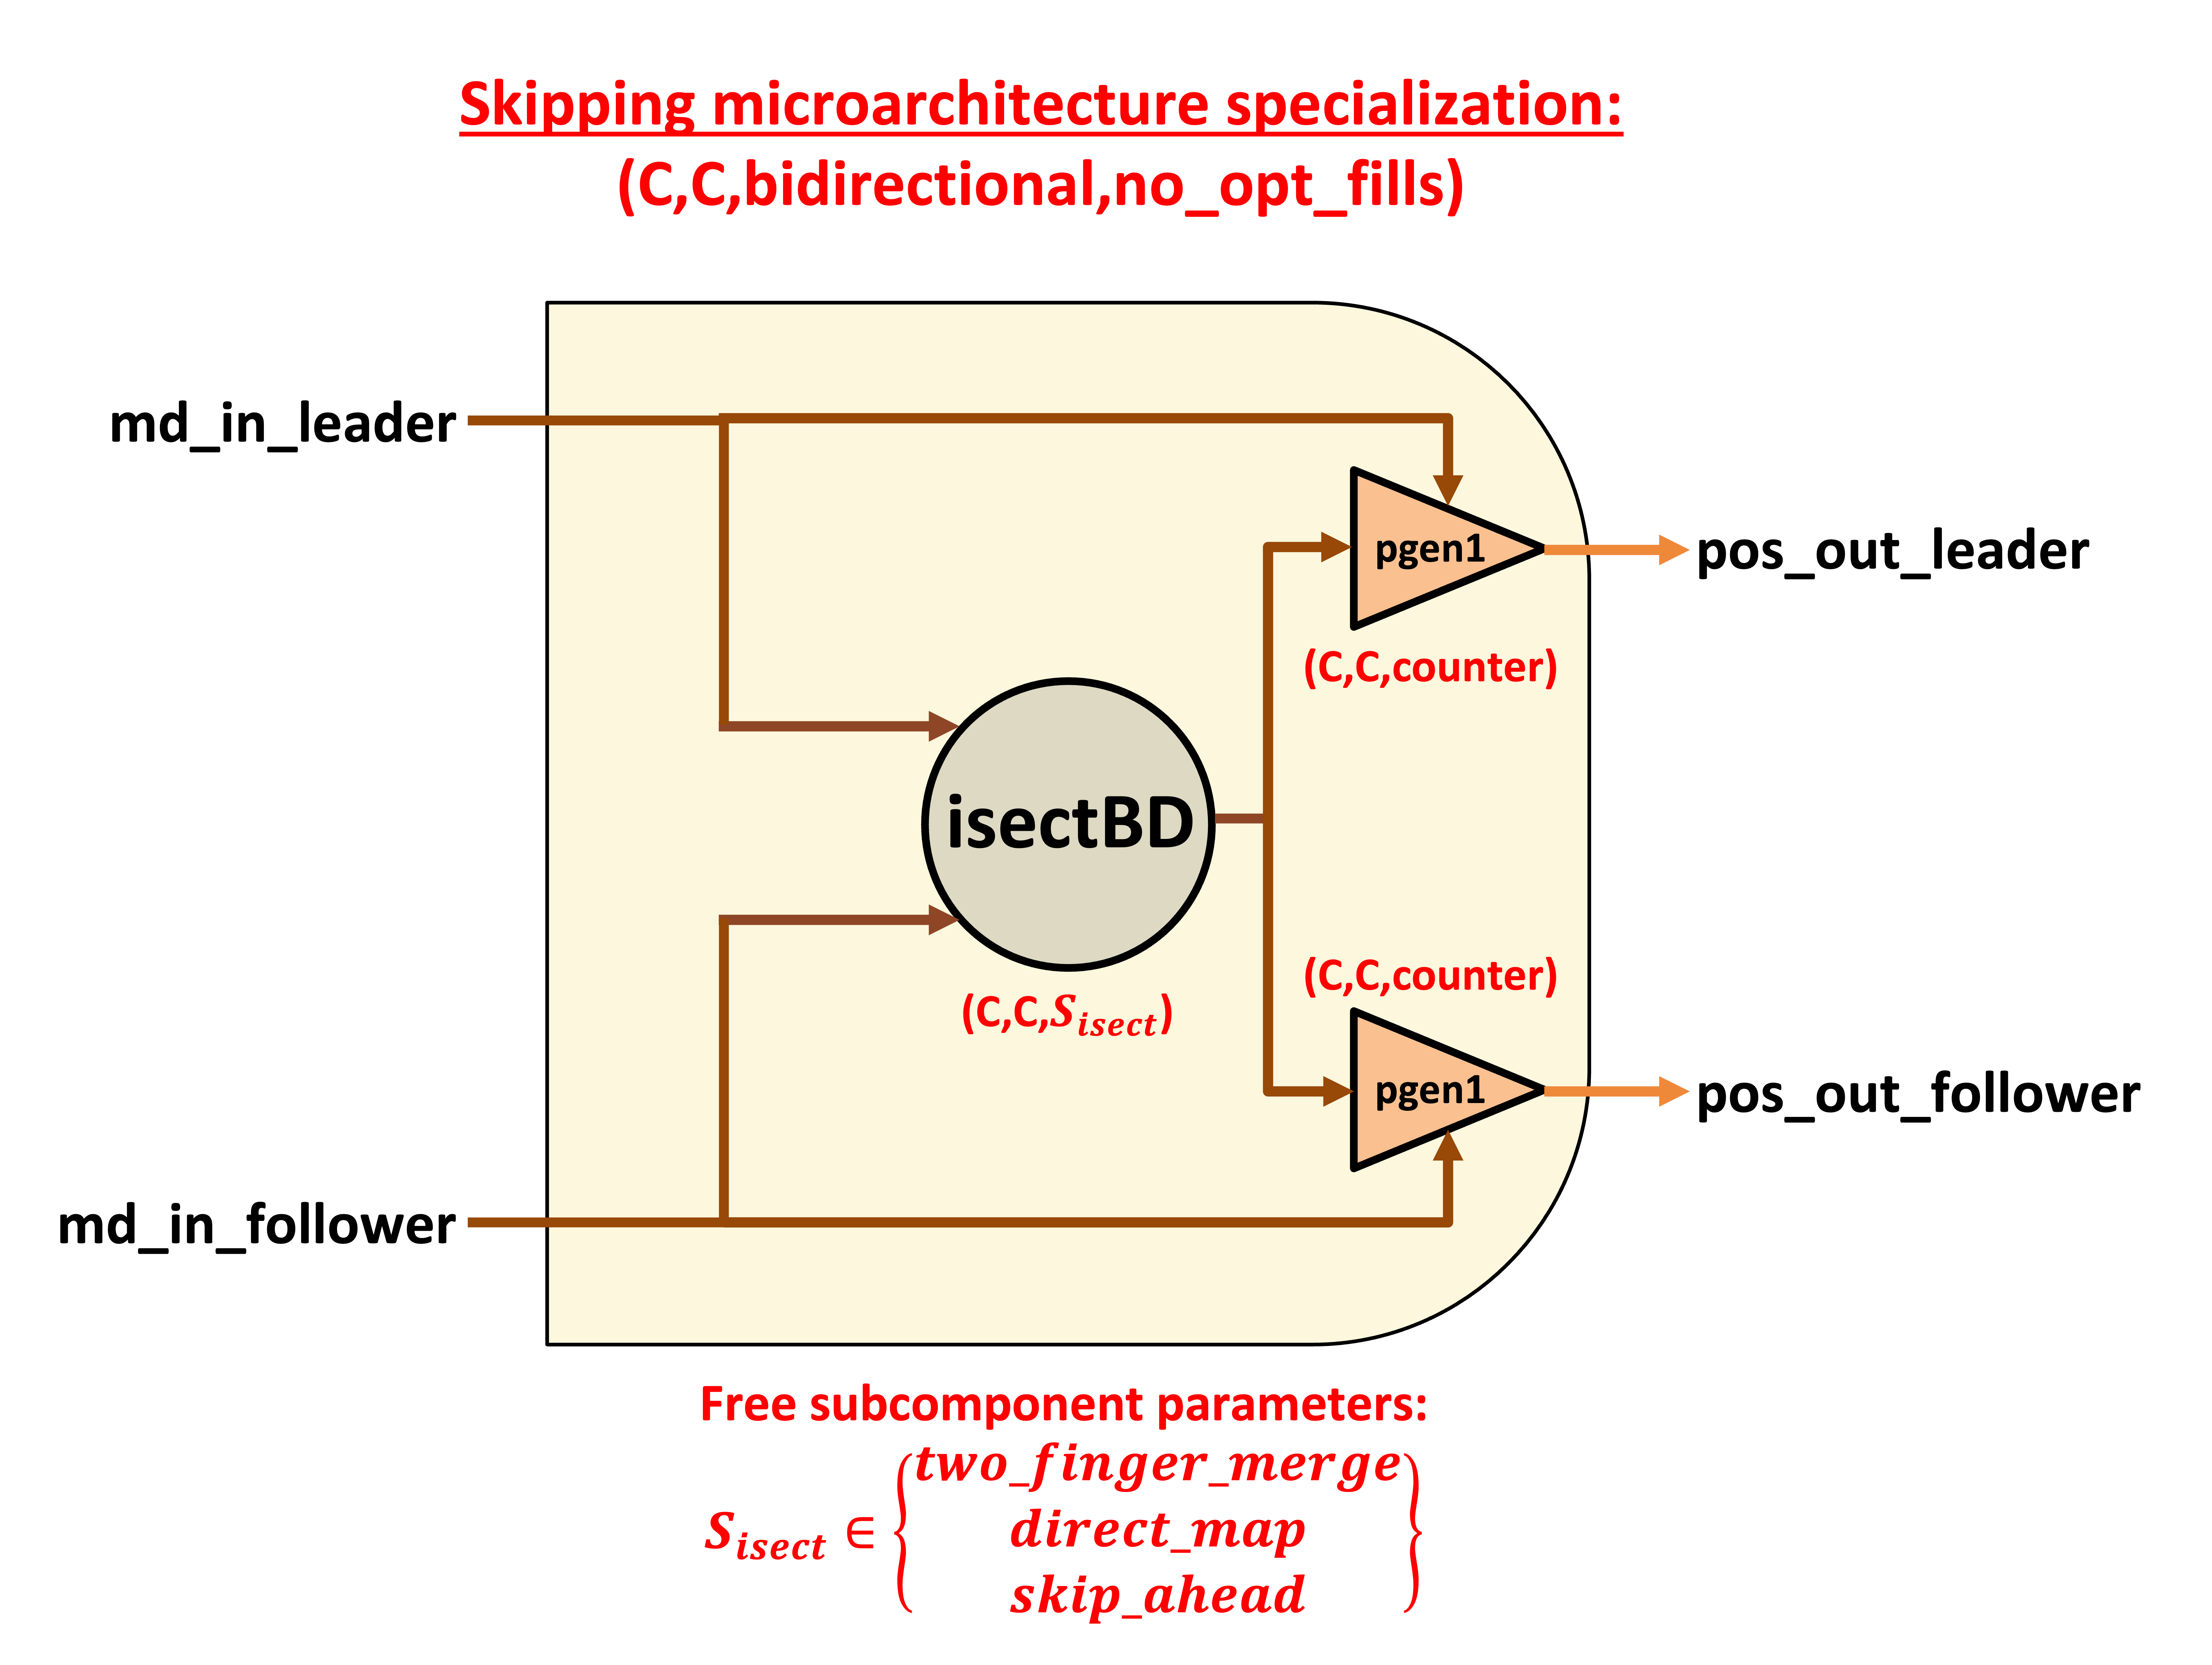
\includegraphics[width=0.95\textwidth]{figures/SKIP_C_C_bidirectional_no_opt_fills.png}
    \caption{Bidirectional coordinate-payload (C) skipping microarchitecture implementation topology (``ExTensor-like''\cite{extensor}.)}
    \label{fig:SKIP_C_C_bidirectional_no_opt_fills}
\end{figure}

\begin{figure}[H]
    \centering
    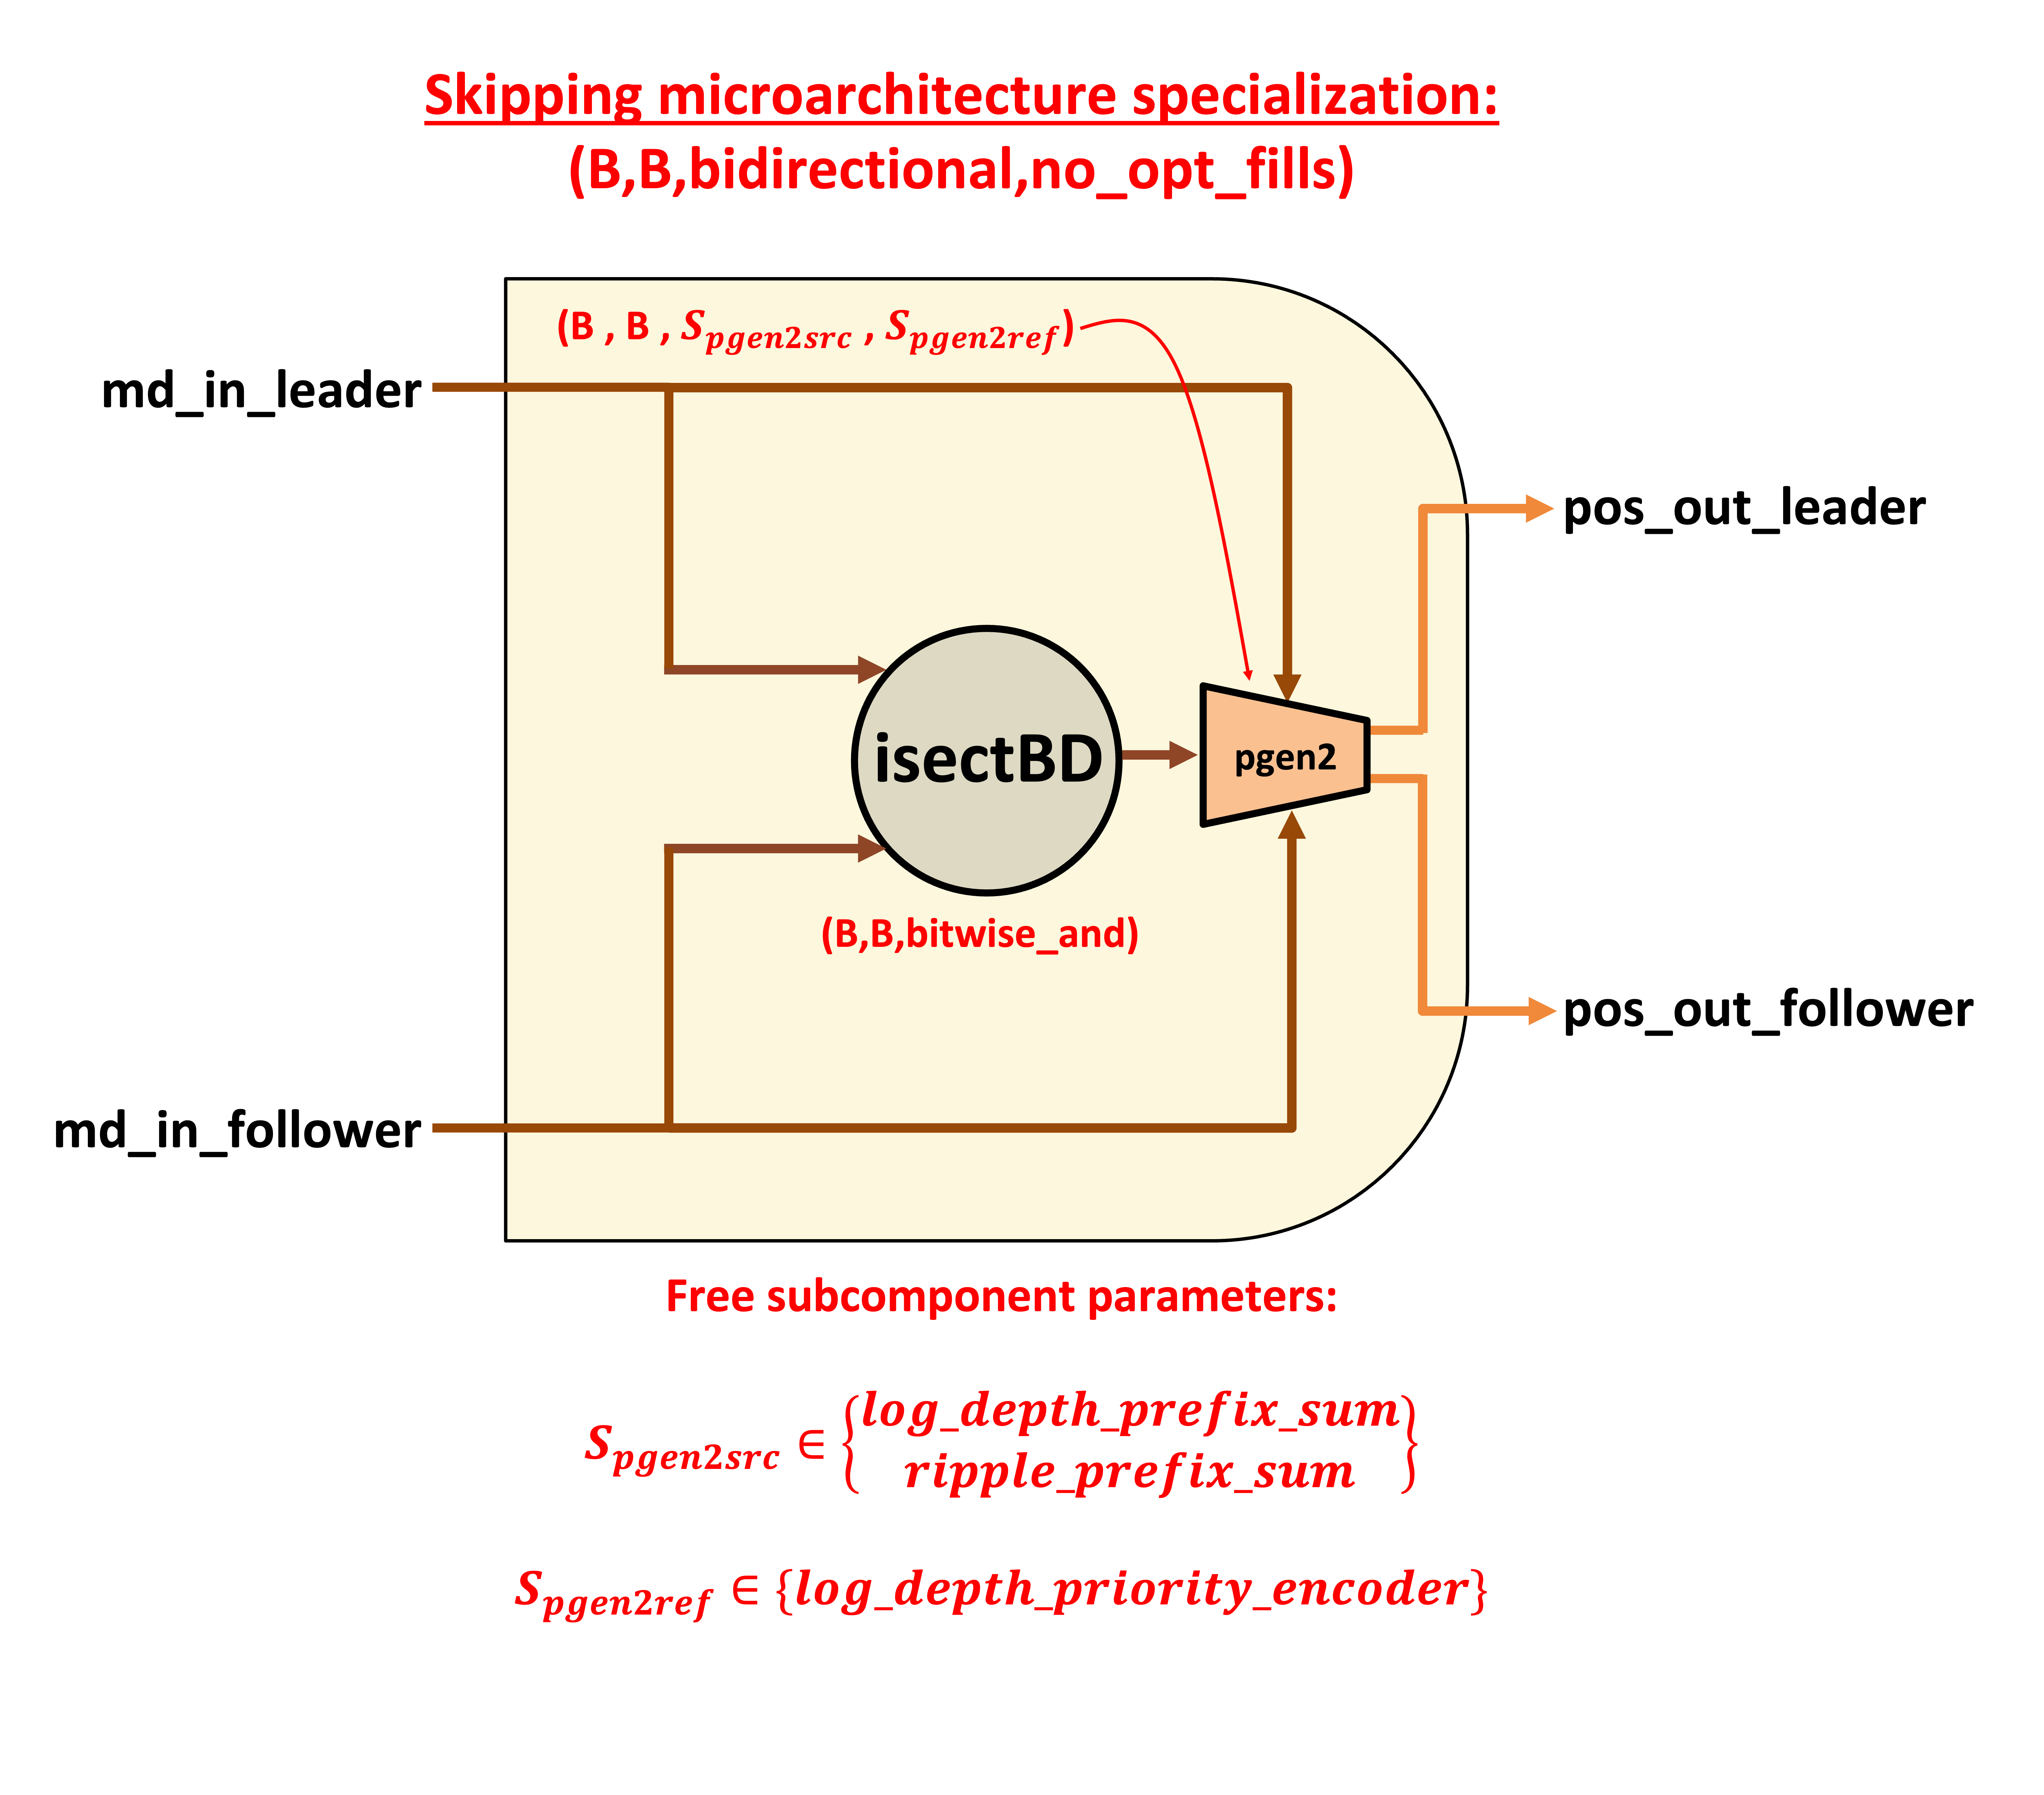
\includegraphics[width=0.95\textwidth]{figures/SKIP_B_B_bidirectional_no_opt_fills.png}
    \caption{Bidirectional bitmask (B) skipping microarchitecture implementation topology (``SparTen-like''\cite{sparten}.)}
    \label{fig:SKIP_B_B_bidirectional_no_opt_fills}
\end{figure}

\begin{figure}[H]
    \centering
    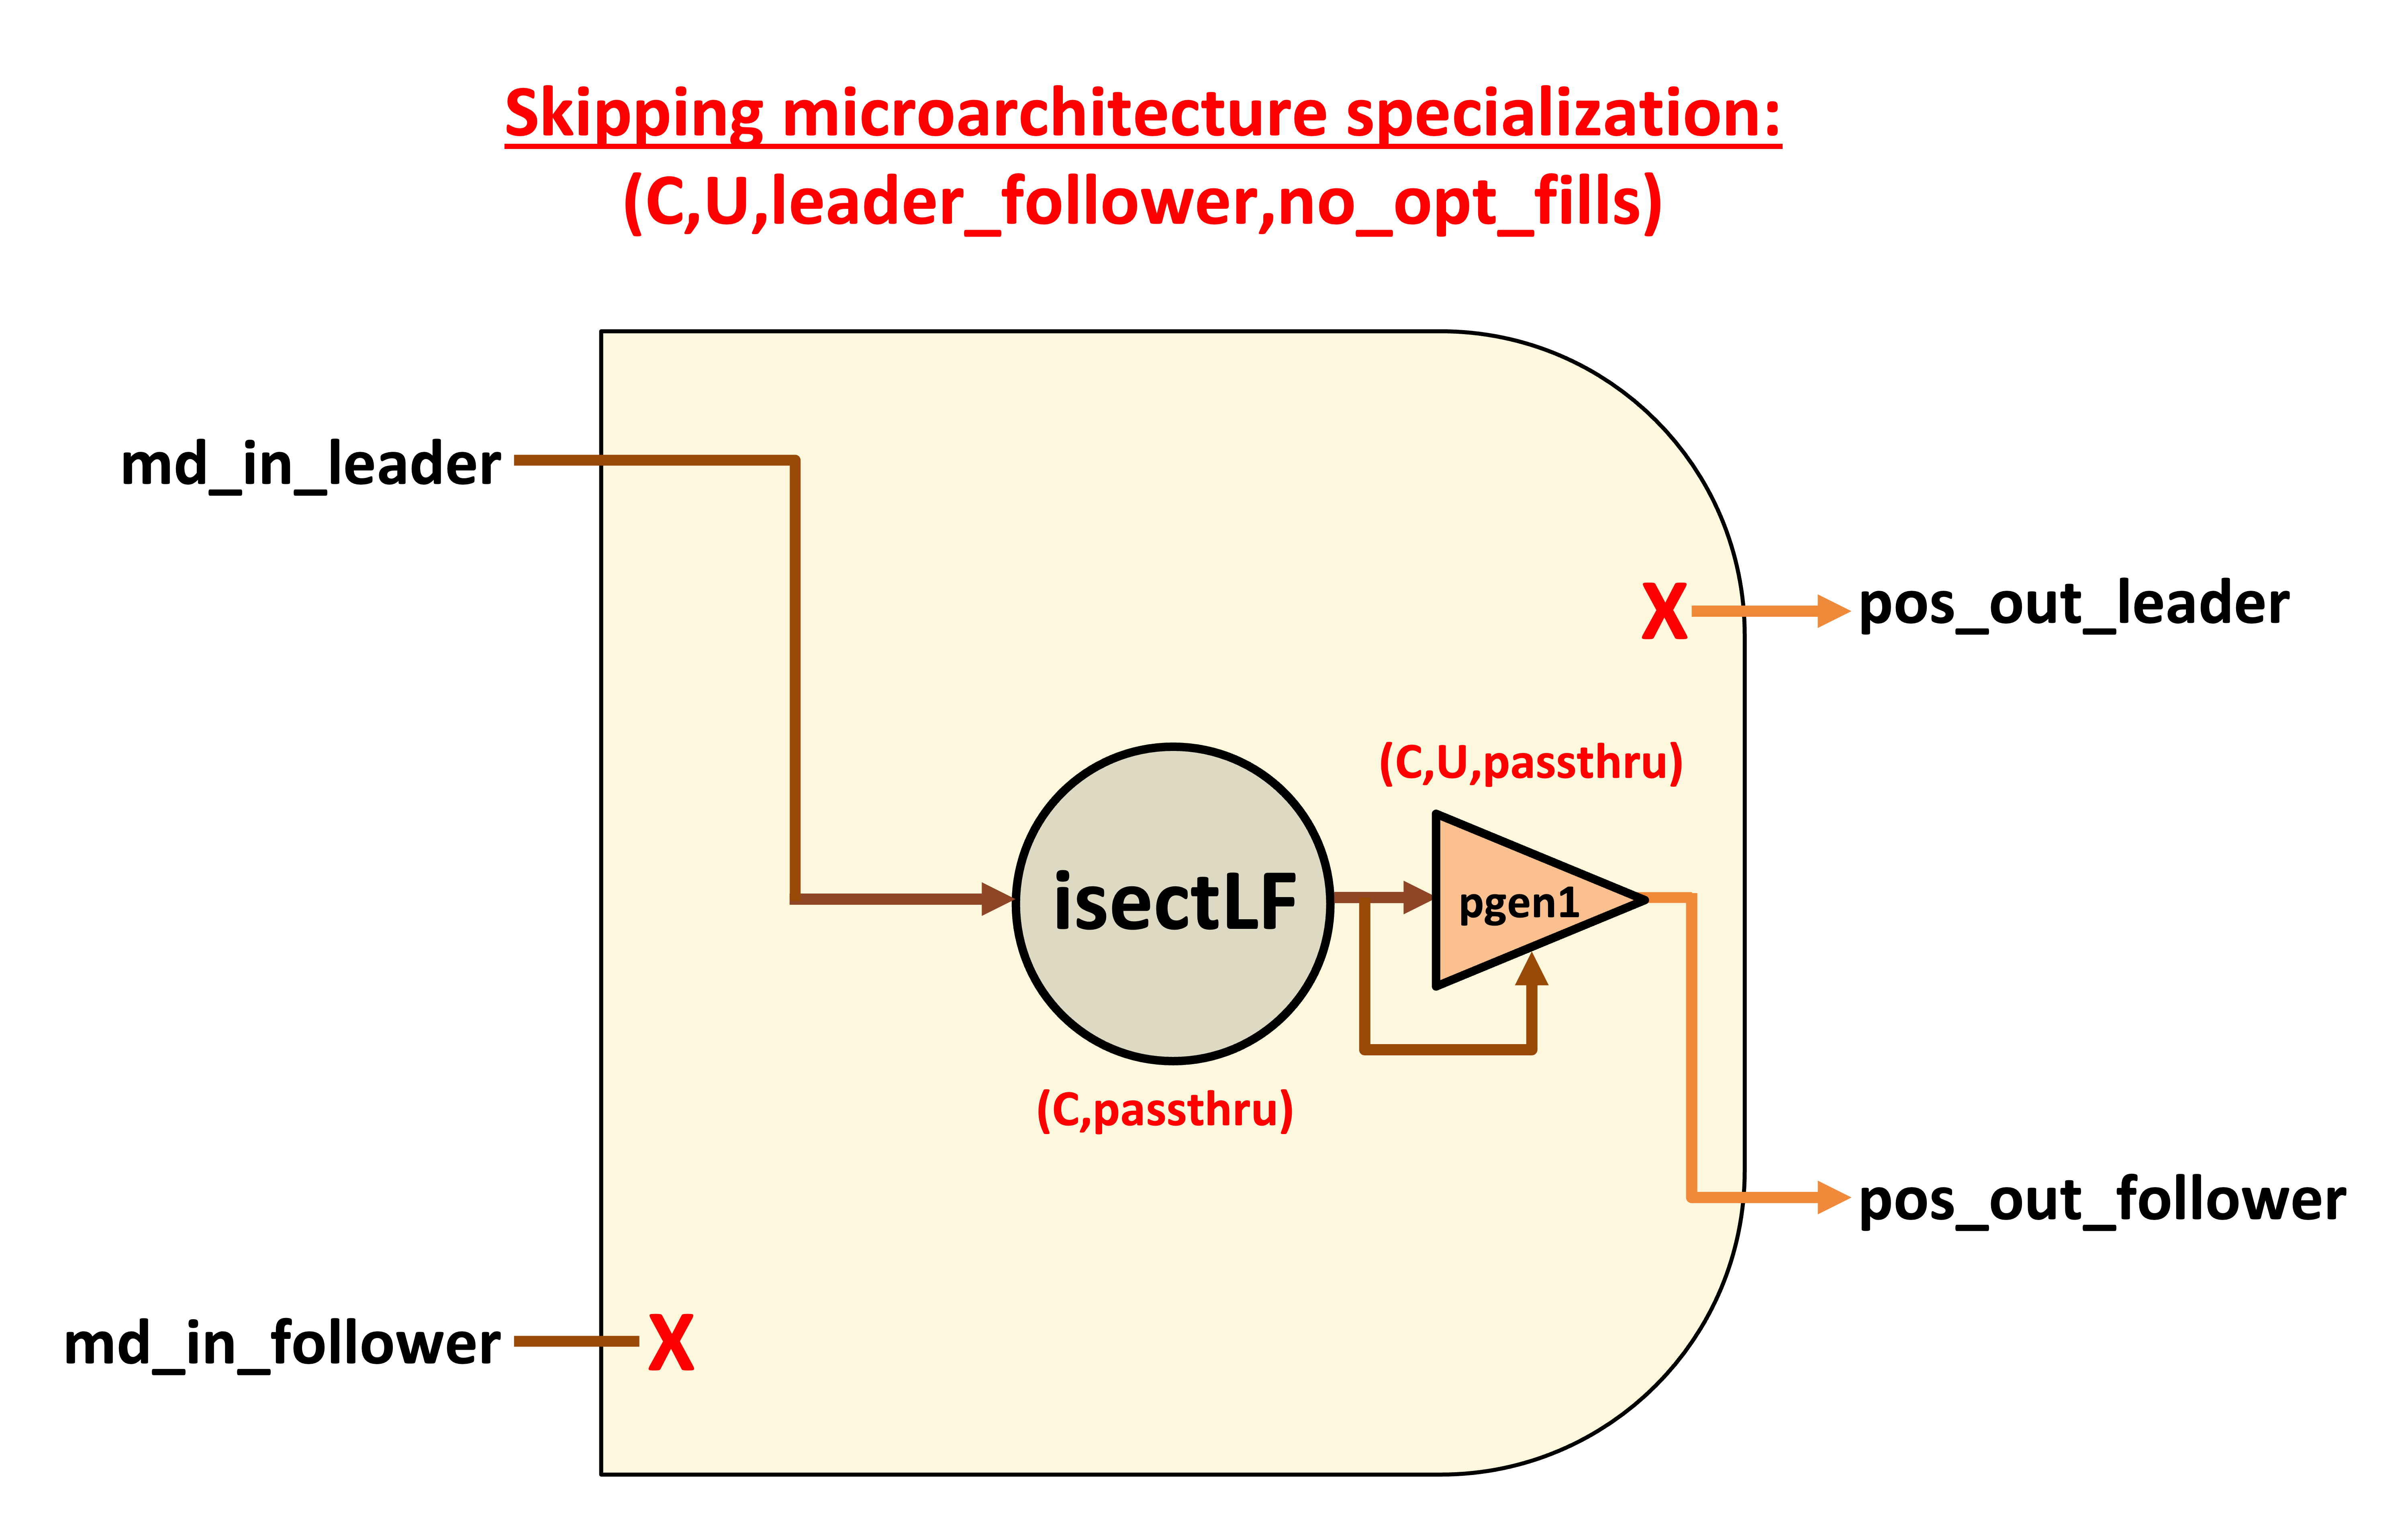
\includegraphics[width=0.95\textwidth]{figures/SKIP_C_U_leader_follower_no_opt_fills.png}
    \caption{Leader-follower coordinate-payload (C) to uncompressed offset-pair (U) skipping microarchitecture implementation topology, without fill optimization.}
    \label{fig:SKIP_C_U_leader_follower_no_opt_fills}
\end{figure}

\begin{figure}[H]
    \centering
    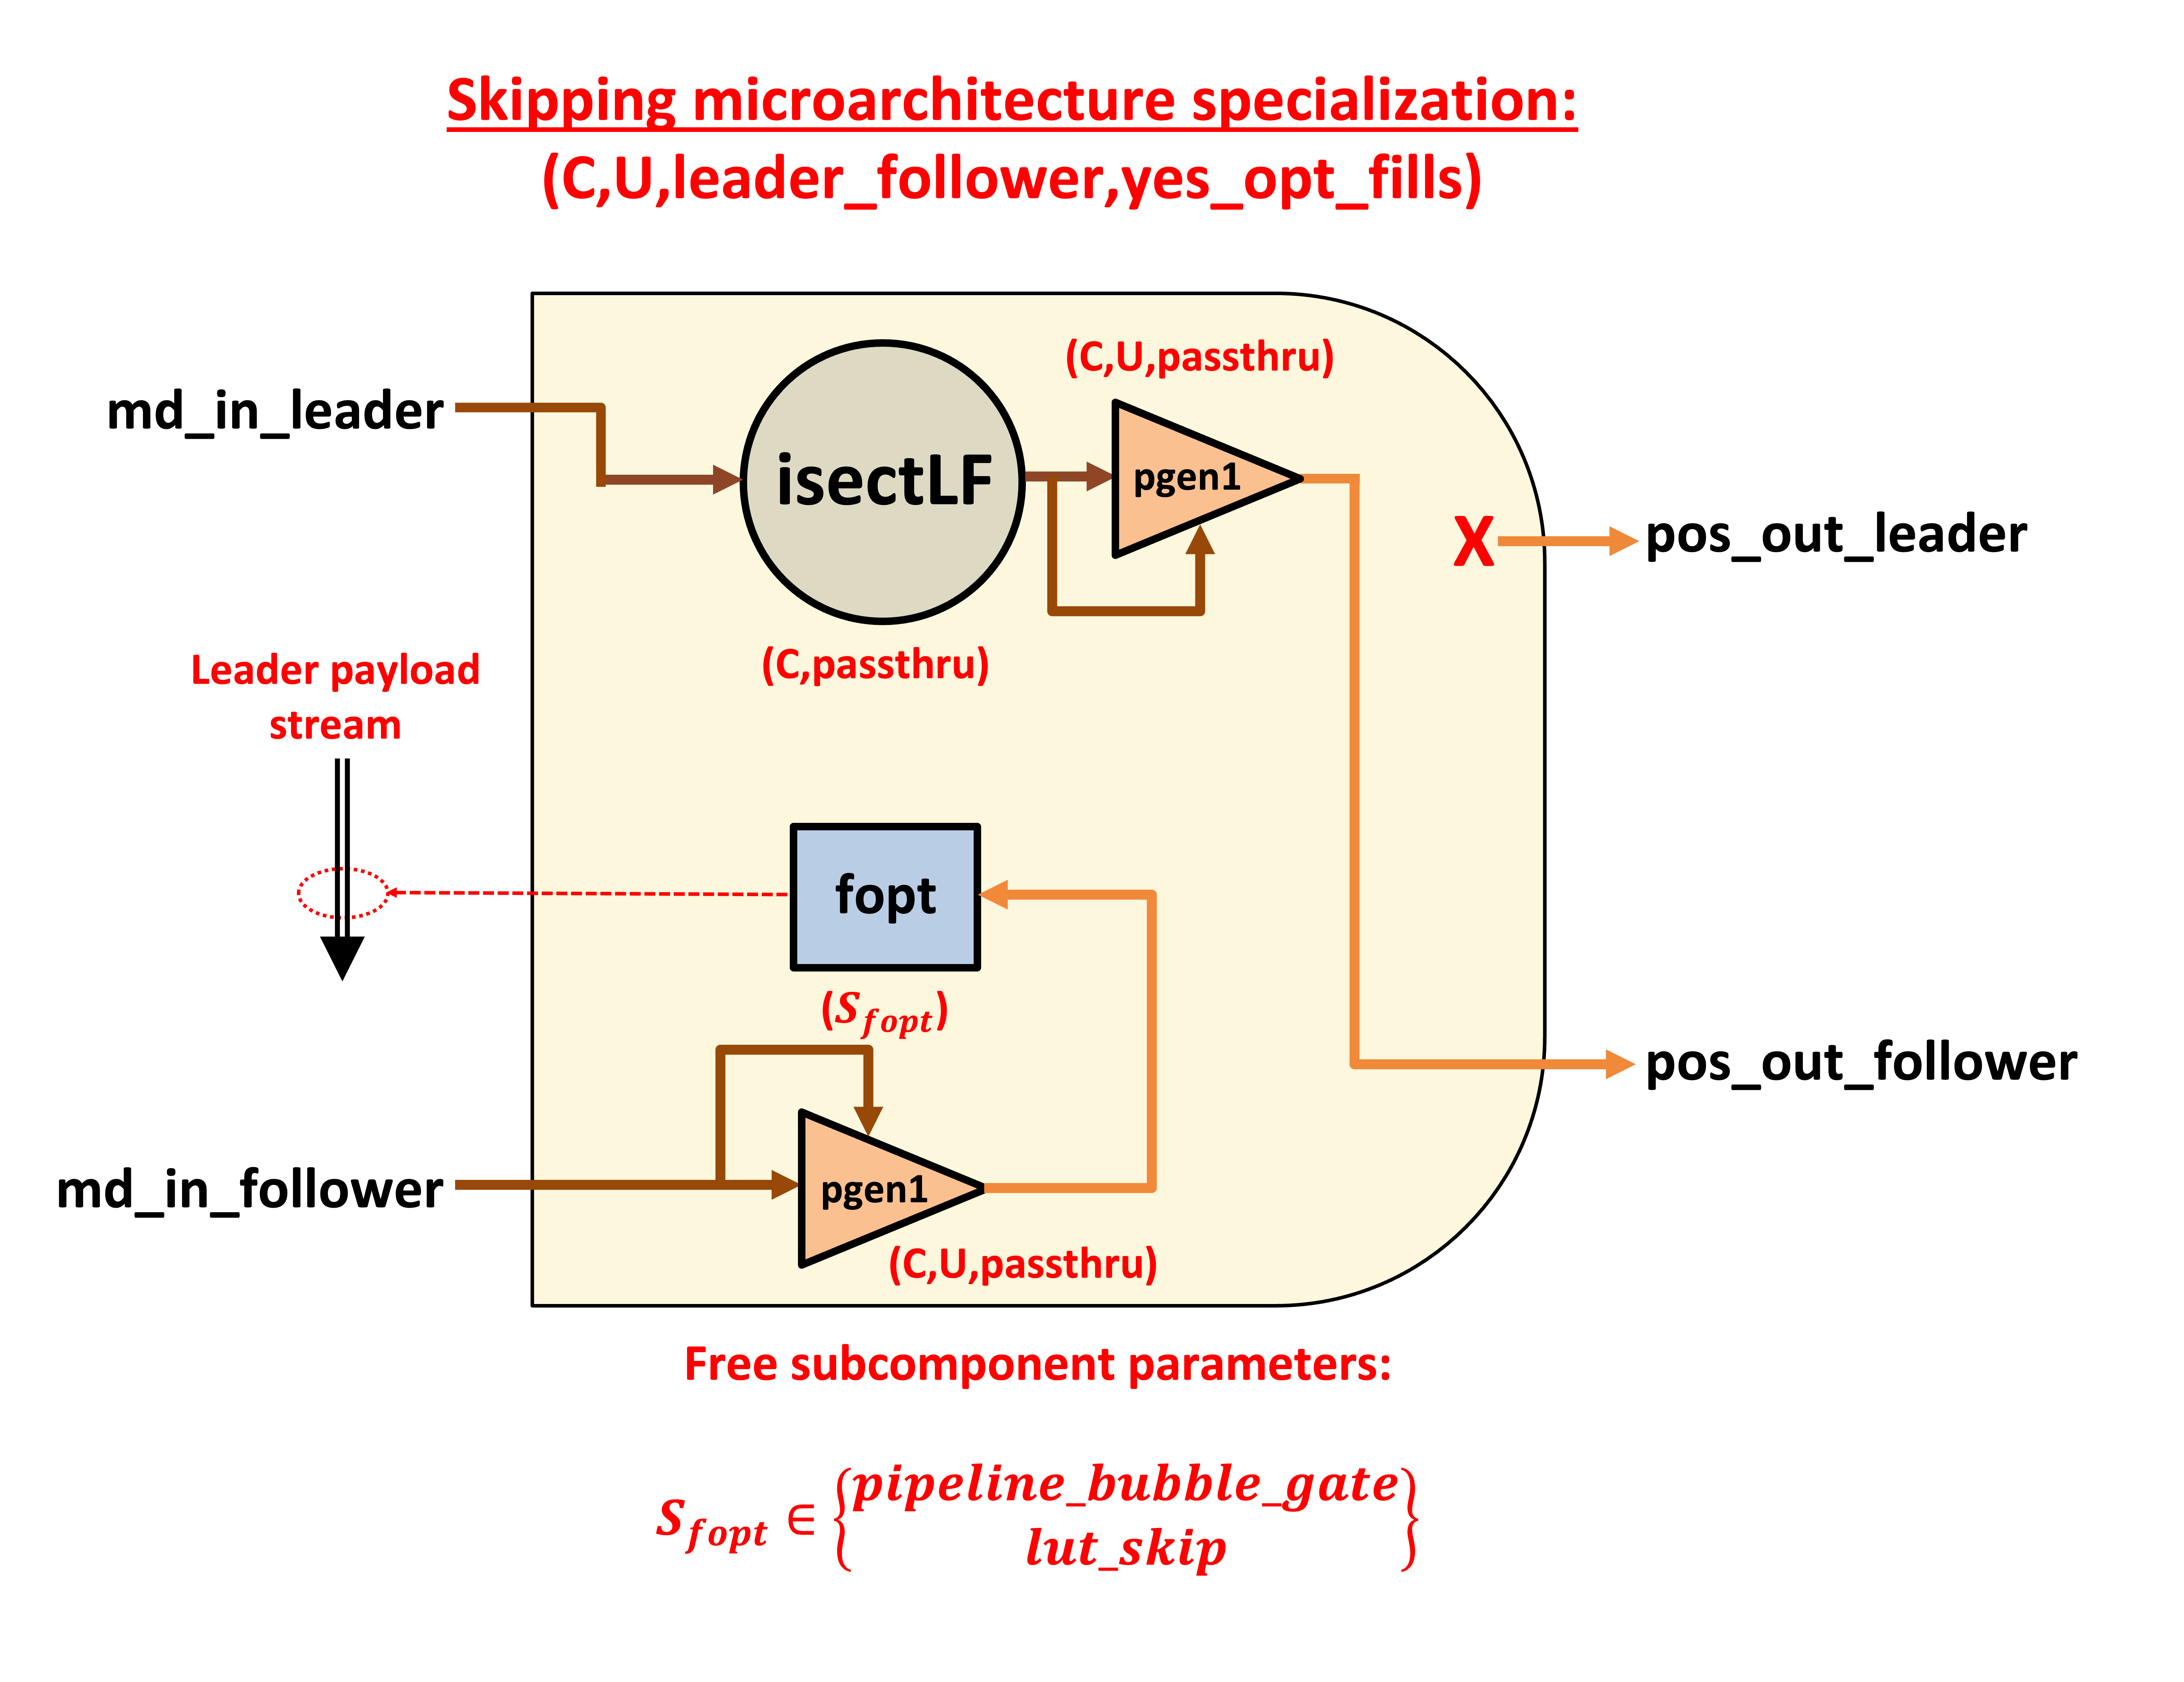
\includegraphics[width=0.95\textwidth]{figures/SKIP_C_U_leader_follower_yes_opt_fills.png}
    \caption{Leader-follower coordinate-payload (C) to uncompressed offset-pair (U) skipping microarchitecture implementation topology, with fill optimization (``Eyeriss-v2-like''\cite{eyerissv2}.)}
    \label{fig:SKIP_C_U_leader_follower_yes_opt_fills}
\end{figure}